\documentclass[oneside]{book}
\usepackage[a4paper, total={6in, 8in}]{geometry}
\usepackage[english]{babel}
\usepackage[utf8]{inputenc}
\usepackage[T1]{fontenc}
\usepackage{cancel}
\usepackage{amsmath}
\usepackage{amsfonts}
\usepackage{dsfont}
\usepackage{listings}
\usepackage{hyperref}
\usepackage{siunitx}
\usepackage{fancyhdr}
\usepackage{textcomp}
\usepackage{makecell}
\usepackage[font=small,labelfont=bf]{caption}
\usepackage{pdfpages}
\usepackage{multicol}
\usepackage[ruled,vlined]{algorithm2e}
\usepackage{soul}
\usepackage{mhchem}
\usepackage[toc, page]{appendix}
\usepackage{float}
\usepackage{wrapfig}
\usepackage{braket}
\usepackage{xcolor}
\pagestyle{fancy}
\fancyhf{}
\lhead{\rightmark}
\cfoot{\leftmark}
\rfoot{\thepage}

\setcounter{secnumdepth}{5}

\lstset{
    frame=tb, % draw a frame at the top and bottom of the code block
    tabsize=4, % tab space width
    showstringspaces=false, % don't mark spaces in strings
    numbers=none, % display line numbers on the left
    commentstyle=\color{green}, % comment color
    keywordstyle=\color{red}, % keyword color
    stringstyle=\color{blue}, % string color
    breaklines=true,
    postbreak=\mbox{\textcolor{green}{$\hookrightarrow$}\space}
}

\renewcommand{\lstlistingname}{}% Listing -> Algorithm
\renewcommand{\lstlistlistingname}{Algoritmi}% List of Listings -> List of Algorithms
\author{
  Giacomo Fantoni \\
  \small Telegram: \href{https://t.me/GiacomoFantoni}{@GiacomoFantoni} \\[3pt]
  Github: \href{https://github.com/giacThePhantom/AlgoritmiStruttureDati}{https://github.com/giacThePhantom/AlgoritmiStruttureDati}}


\renewcommand*{\listalgorithmcfname}{}
\renewcommand*{\algorithmcfname}{}
\renewcommand*{\algorithmautorefname}{}
\renewcommand{\thealgocf}{}
\newcommand{\mathcolorbox}[2]{\colorbox{#1}{$\displaystyle #2$}}


\title{\Huge \textbf{Molecular Physics}}

\author{
  Giacomo Fantoni \\
  \small Telegram: \href{https://t.me/GiacomoFantoni}{@GiacomoFantoni} \\[3pt]
  Ilaria Cherchi\\
  \small telegram: \href{https://t.me/ilariacherchi}{@ilariacherchi} \\[3pt]
  Alessia Guadagnin\\
  \small telegram: \href{https://t.me/alessiagp}{@alessiagp} \\[3pt]
\small Github: \href{https://github.com/giacThePhantom/MolecularPhysics}{https://github.com/giacThePhantom/MolecularPhysics}}
\begin{document}
\maketitle
\tableofcontents

  \part{Quantum mechanics}

    \chapter{Revisiting classical mechanics}

\section{Physical theories}

  \subsection{Experiment}
  An experiment performed on a physical system is a way to measure observable quantities at a determined time: $O_1(t), \dots, O_n(t)$.
  By measuring more and more observables at the same time, the instantaneous state of the system becomes increasingly characterized.
  A maximum set of observables that leads to the complete characterization of the instantaneous state can be assumed.

    \subsubsection{Example - particle of mass $m$ subject to an harmonic force}
    A particle of mass $m$ subject to an harmonic force like one of a spring is completely characterized by: 
    
    $$(\vec{r}(t),\vec{v}(t))=\vec{r}(t)\in \mathbb{R}^6$$

  \subsection{Definition}
  A physical theory is a mathematical scheme to predict the state of the system, the outcome of feature observations: $O_1(t'), \dots, O_n(t')$.
  In particular, an equation that can be used to compute the state at $t'$ given the state at $t$ is called an equation of motion.
  A physical theory is composed by the following elements:
  \begin{itemize}
    \item definition of the state of a system
    \item recipe to determine the system's equation of motion
    \item prediction of an observable quantity given the state of the system
   \end{itemize}
   

\section{Classical mechanics}
In classical mechanics, the state of a system is a collection at time $t$ of all the positions of all the particles in the system. We also need to define the velocity of the particle, or, better, the momentum - which is obtained by scaling the velocity by a constant in classical mechanics, so the two are equivalent. The mathematical tool that allows us to understand how a state evolves in time is the time derivative of the equation of interest (differential equation).

  \subsection{Newtonian mechanics}
  Newtonian Mechanics is a theory described by the three Newton's laws, which are in principle well stated:
  \begin{enumerate}
    \item a body will continue its state at rest or at constant speed unless a force acts. Loophole: it is only true in inertial frames. The lack of an initial consensus inertial frames raises issues.
    \item how does the body change when it is subject to a force. Loophole: but what is a force? Here we only deal with mass and acceleration. We have an issue, stuck in a loop.
    \item whenever A acts on B, B acts on A with opposite sign (action-reaction)
  \end{enumerate}
  
  Hamilton's function is a function of position and momentum. 
  $$H(\underbrace{\vec{p}}_{\text{momentum}}, \underbrace{\vec{q}}_{\text{position}}) = \frac{\vec{p}^2}{2m} + U(\vec{q})$$
  The first term is the kinetic energy, while the second term is the potential energy (scalar function of position). Remember that what we are after is   a rigorous definition; since kinetic energy is given, we only need to specify the potential energy. The derivative of the position will be the derivative of H with respect to position.
Are Hamilton's equation really consistent with Newton's equations? Indeed, from H(p,Q) we can retrieve Newton's equations of motion, solve them, get predictions and compare with experimental results. The workflow is the following:
\begin{itemize}
    \item define H
    \item compute equation of motion
    \item solve equation of motion
    \item use solution to obtain predictions of experimentally observable quantities
    \item experimentally test the prediction (yes/no)
\end{itemize}
The procedure is repeated until concordance with experiments is reached. But we never defined force, we only deal with H!

  \subsection{Example - point particle moving in $1D$ and subject to an harmonic force}
  For a point particle moving in $1D$ subject to an harmonic force (bound to a spring for example) follows the Newton's law for its equation of motion:

  $$\frac{d{^2}}{d{t^2}}x(t) = -\frac{k}{m}x(t)$$

  If, given $\lambda$ the amplitude, $L$ the oscillation and $L_0$ the distance of the point from the origin of the axis at time $0$:

  \begin{multicols}{3}
    \begin{itemize}
      \item $\frac{\lambda}{L}\ll 1$
      \item $\frac{\lambda}{L_0}\ll 1$.
      \item $\frac{L}{L_0}\ll 1$.
    \end{itemize}
  \end{multicols}

  This is a second-order differential equation such that $\frac{d{^2}}{d{t^2}}f(t) = -\frac{k}{m}f(t)$.
  There are only two solutions:

  \begin{align*}
    f_1(t) = \sin(\omega t) &\Rightarrow \frac{d{^2}}{d{t^2}}f)1(t) = -\omega^2f_1(t)\\
    f_2(t) = \cos(\omega t) &\Rightarrow \frac{d{^2}}{d{t^2}}f)2(t) = -\omega^2f_2(t)\\
  \end{align*}

  Clearly, $f_1(t)$ and $f_2(t)$ are solutions if $\omega^2 = \frac{k}{m}$.
  Neither of them is a good solution: the first one is only valid if the particle starts at the origin, while the second one only holds if the particle is at rest at time $0$.
  So the most general solution is:

  $$x(t) = A\cos\sqrt{\frac{k}{m}}t+B\sin\sqrt{\frac{k}{m}}t$$

  To find $A$ and $B$, information about the initial conditions are used.
  Let the initial position $x(0) = x_0$.
  Then 

  $$x(0) = A = x_0$$

  Considering initial velocity: $\frac{d{}}{d{t}}x(t)|_{t=0} = v_0$, then:

  \begin{align*}
    \frac{d{}}{d{t}}x(t) &= -\sqrt{\frac{k}{m}}A\sin\sqrt{\frac{k}{m}}t + \sqrt{\frac{k}{m}}B\cos\sqrt{\frac{k}{m}}t\\
    v_0 &= \sqrt{\frac{k}{m}} B \Rightarrow B = \sqrt{\frac{m}{k}}v_0
  \end{align*}

  So the final solution is:

  $$\begin{cases}
    x(t) = x_0\cos\sqrt{\frac{k}{m}}Bt+\sqrt{\frac{m}{k}}v_0\sin\sqrt{\frac{k}{m}}t\\
    v(t) = v_0\cos\omega t -x_0\omega\sin\omega t
  \end{cases}$$

  \subsection{Phase-space}
  It is convenient to plot the solutions on the phase space, a plane such that on the $x$-axis there is the position $x=q(t)$ and on the $y$-axis the momentum $m\times v=p(t)$.
  In this way the state of the system will be described as:

  $$\Gamma(t) = (q(t),p(t))$$

  Cauchy's theorem implies that given a n-th order differential equation and given $n$ initial conditions, there exists exactly one solution.
  Because of this, trajectories in the phase space can never intersect (corollary).
  Classical mechanics is fully deterministic, as future $x(t)$ and $v(t)$ can be unambiguously predicted. 

  \subsection{Systems in three dimension and with more than one particle}
  For systems with $D=3$ and for more than one particle the equation of motion is:

  $$\begin{cases}
    m_1 \frac{d{^2}}{d{t^2}}\vec{r}_1(t) = \vec{F}_1(\vec{r}_1(t), \dots,\vec{r}_N(t))\\
    \vdots\\
    m_N \frac{d{^2}}{d{t^2}}\vec{r}_N(t) = \vec{F}_N(\vec{r}_1(t), \dots,\vec{r}_N(t))\\
  \end{cases}$$

  Correspondingly, the phase-space is $6N$ dimensional.
  Moreover, for the $N$ vector equations there are $N$ scalar ones.

  \subsection{Work and energy}
  Let $\vec{r}$ be a trajectory followed by a particle subject to a force $\vec{F}$.
  The work of the force $\vec{F}$ from point $A$ to point $B$ of the trajectory is defined as:

  $$W_{AB} = \int_{\vec{r}_a}^{\vec{r}_b}d \vec{r}\cdot \vec{F}$$

  The kinetic energy of the particle is instead:

  $$T = \frac{1}{2}mv^2$$

  Work and energy are related:

  \begin{align*}
    \frac{d{}}{d{t}}T = \frac{d{}}{d{t}}\frac{1}{2}mv^2 = \frac{1}{2}m \frac{d{}}{d{t}}v^2 = \frac{1}{2}2m \vec{v}\underbrace{\frac{d{\vec{v}}}{d{t}}}_{\vec{a}} = \vec{v} \vec{F}\\
    \int_{t_0}^{t_f}dt \frac{d{}}{d{t}}T = T_B-T_A = int_{t_i}^{t_f}dt \frac{d{\vec{r}}}{d{t}}\vec{F} = \int_{\vec{r}_A}^{\vec{r}_B} d \vec{r}\cdot \vec{F} = W_{AB}\\
    T_B-T_a = W_{A\rightarrow B}
  \end{align*}

    \subsubsection{Conservative forces}
    For conservative forces, the work from point $A$ to point $B$ does not depend on the path followed. In particular, for each path $1$ and $2$: $W_{AB}^1 = W_{AB}^2$ and:

    $$-W_{AB} = U(\vec{r}_B) - U(\vec{r}_A)$$

    Where $U(\vec{r})$ is the potential energy.
    In one dimension:

    \begin{align*}
      U(r) -U(r_0) = -w_{x_0x} = -int_{x_0}^xdyF(y) \Rightarrow\\
      -\frac{d{}}{d{x}}U(x) = F(x)
    \end{align*}

      \paragraph{Three dimensional case}
  
      $$\begin{cases}
        F_x(x,y,z) = - \frac{\partial {}}{\partial {x}}U(x,y,z)\\
        F_y(x,y,z) = - \frac{\partial {}}{\partial {y}}U(x,y,z)\\
        F_z(x,y,z) = - \frac{\partial {}}{\partial {z}}U(x,y,z)\\
      \end{cases}$$
  
      Or, in short hand notation, let $\vec{r}=(x,y,z)$ and $\vec{\nabla}(\frac{\partial {}}{\partial {x}},\frac{\partial {}}{\partial {y}},\frac{\partial {}}{\partial {z}})$, then:
  
      $$\vec{F}(\vec{r}) = -\vec{\nabla}U(\vec{r})$$
  
      \paragraph{Central forces}
      Central forces are a notable class of conservative forces, for which $\vec{F}(\vec{r}) = \hat{\omega}_{r}f(r)$ and $\vec{r} = \hat{U}_{r}|\vec{r}| = \hat{U}_{r}r$.
      Some examples:

      \begin{multicols}{2}
        \begin{itemize}
          \item Coulomb: $\vec{F}_e = \hat{U}_{\vec{r}}\frac{q_1q_2}{r_{12}^2}$
          \item Gravity: $\vec{F}_G = -\hat{U}_r\frac{M_1M_2}{r_{12}^2}G$
          \item Harmonic $\vec{F} = -\hat{\omega}_r(\vec{r}-\vec{r}_0)$
          \item $\cdots$
        \end{itemize}
      \end{multicols}

  \subsection{Conservation of mechanical energy}
  Reconsidering the relationships between $T$ and $W$:

  $$T_B-T_A = W_{A\rightarrow B} = U_A-U_B$$

  The mechanical energy $H$ can be introduced, such that:

  $$H_A = T_A+U_A = T_B+U_B = H_B$$

  The mechanical energy is conserved in the system only if conservative forces act on it.
  Energy conservation allows us to solve Newton's equation, which is generally impossible to handle.
  This is because conservation laws help gaining partial information without having to solve Newton's equation.
  At this level, energy conservation comes in as a matter of convenience.

    \subsubsection{Example}
    Consider a cart going down a path with a loop.
    Let $A$ be the starting highest point when it starts going and $B$ the lowest point where it stops accelerating.

    $$\begin{cases}H_A = \underbrace{T_A}_{=0}+\underbrace{U_A}_{=mgh}\\
    H_B = \underbrace{T_B}_{-\frac{1}{2}mv^2}+\underbrace{U_B}_{=0}\end{cases}
    \Rightarrow v = \sqrt{2gh}$$

  \subsection{Angular momentum conservation}
  Let the angular momentum:

  $$\vec{L}(t) = \vec{r}(t)\times m \vec{v}(t)$$
 The angular momentum is also defined as the vector product of the particle position and its linear momentum. 
 $$\vec{L}=\bar{x} \times \bar{P}$$ \\
  There are two ways to solve a cross product: $\vec{a}\times \vec{b}\perp \vec{a}$, $\vec{a}\times \vec{b}\perp \vec{b}$ and $|\vec{a}\times \vec{b}| = |\vec{a}||\vec{b}|\sin\theta$.
  This implies that $\vec{a}\parallel \vec{b}\Rightarrow \vec{a}\times \vec{b} = 0$.
  
  Youtube:
  By taking the derivative of the angular momentum with respect to time, we can asses under which conditions linear momenutm is conserved.. The velocity and momentum are parallel, therefore the cross product depending on the angle between them is zero. 
  
  $$\frac{d \vec{L}}{d t}=\frac{d \bar{x}}{d t} \times \vec{p}+\bar{x} \times \frac{d \vec{p}}{d t}=\underbrace{\bar{v} \times \bar{p}}_{0}+m \frac{d \bar{v}}{d t} \Rightarrow \vec{F}=m \cdot \bar{a}$$

$$
\frac{d}{d t} \bar{p}_{+0 r}=\frac{d}{d t}\left(\sum_{i=1}^{N} \bar{p}_{i}\right)=0 \\
m \bar{v}+m \vec{v}=m \bar{v}^{-}+M \vec{v}^{0} \\
\vec{v}^{\prime}=-\left(\frac{m}{M}\right) \bar{v}^{\prime}$$
Whenever the torque of a particle is zero, then the angular momentum of that particle is conserved (centripetal/centrifugal force).
$$\frac{d \vec{L}}{d t}=\bar{x} \times \vec{F}=0 \\
\frac{d}{d t}\left(\vec{L}_{\text {TOT }}\right)=\frac{d}{d t}\left(\Sigma_{i} \vec{L}_{i}\right)=0 \\
$$
  
  Lecture:
  Now considering the vectors' coordinates:

  $$\vec{a}\times \vec{b} = \hat{i}(a_yb_z - a_zb_y) + \hat{j}(a_xb_z - a_zb_x) + \hat{k}(a_xb_y-a_yb_x)$$

  Now considering:

  \begin{align*}
    \frac{d{}}{d{t}}\vec{L} &= \frac{d{}}{d{t}}(\vec{r}\times \vec{p}=\\
                            &=\underbrace{\frac{d{\vec{r}}}{d{t}}}_{=0}\times\vec{p} + \underbrace{\frac{d{\vec{p}}}{d{t}}}_{=F}\times\vec{r} =\\
                            &= \vec{r}\times \vec{F}
  \end{align*}

  If $\vec{r}\parallel \vec{F}\Rightarrow \frac{d{}}{d{t}}\vec{L} = 0$.
  Therefore, for a conservative force there is angular momentum conservation.
  Summarizing, the motion in a central force conserves energy and angular momentum.

\section{Classical theory of the hydrogen atom}
The classical theory of the hydrogen atom is defined by the classical Bohr model.
The hydrogen atom is formed by a proton in the centre with an electron orbiting around it.
Approximations:
\begin{itemize}
  \item the mass of the electron divided by the mass of the proton is around 1/2000 ($\frac{m_e}{M_p}\approx \frac{1}{2000}$). The center of mass of the system is very close to the nucleus, therefore we can assume that the nucleus remains still. For the sake of simplicity an infinite proton mass $\frac{m_e}{M_p}=0$ is assumed.
  \item the charge of the proton is the negative of the charge of the electron, so the overall system is neutral
  \item  Because $\frac{d{}}{d{t}}\vec{L}=0$ (angular momentum conservation), the electron's motion occurs on a plane and is two dimensional.
\end{itemize}
Let us start from the Newton's equations. We wish to express the attracting force acting on the electron towards the proton (inward direction, negative sign). Since x,y,z are varying with time (as the electron is moving) we can express them as $x(t)$,$y(t)$ and $z(t)$. The equations are coupled, meaning that we cannot solve one at a time e.g. we require $y(t)$ and $z(t)$ for solving the first one, the same applies to the others.
This is a quite tricky task, but luckily there is a way round this problem. We can employ the energy conservation that we mentioned previously though the usage of polar coordinates.

In this case we have a position vector $r$ going from the proton to the electron. The Coulombic force has a specific feature: it points on the same line of the position, radial centripetal force. The important aspect is that $F$ is parallel to $r$. The mathematical expression shows that forces are anti-parallel. Rather than using cartesian coordinates, we can use rotating coordinates. The centrality of force will imply two main results: mechanical energy is conserved and the angular momentum  of the particle is ... the torque, but it is zero for centripetal force, i.e. L is conserved.
The second considerations lead us to understand that orbit lines are confined on a plane. This is particularly relevant, as in a plane we only need two coordinates- as the third coordinate is fixed to zero.

  \subsection{Mechanical energy in polar coordinates}

  $$H = \underbrace{\frac{p^2}{2m}}_{\text{kinetic energy}}-\underbrace{\frac{e^2}{r}}_{\text{potential energy}}$$

  The potential energy is derived from Coulomb's $F=-\hat{r}\frac{e^2}{r^2}$, so $U(|\vec{r}|) = -\frac{e^2}{|\vec{r}|}$


  Now, by using conservation to replace the differential equation, the position is divided in two components $\hat{u}_r$ and $\hat{u}_\theta$ orthogonal to each other, so that $v^2 = v_r^2+v_\theta^2$:

  $$\vec{v} = \hat{u}_\theta v_\theta +\hat{u}_r\underbrace{v_r}_{\frac{d{r}}{d{t}}}\Rightarrow v_2 = \biggl(\frac{d{r}}{d{t}}\biggr)^2+v_\theta$$

  Now, rewriting the angular momentum:

  \begin{align*}
    \vec{L} = m \vec{r}\times(\underbrace{\vec{v}_r}_{=0}+\vec{v}_\theta) &= m \vec{r}\times\vec{v}_\theta\\
    |L| &= mrv_\theta\\
    L^2 = m^2r^2v^2
  \end{align*}

  Substituting this in the Hamiltonian:

  \begin{align*}
    H &= \frac{1}{2}mv_r^2 + \frac{1}{2}mv_\theta^2 - \frac{e^2}{r}=\\
      &=\frac{1}{2}mv_r^2 + \underbrace{\frac{L^2}{2mr^2}}_{\text{Simil-potential, L constant}} - \frac{e^2}{r}
  \end{align*}
  
  This term depends on $r$ and not on $\theta$ and effectively looks like a potential energy.
  So $\frac{L^2}{2mr^2}-\frac{e^2}{r}\equiv V_{eff}(r)$.
  And:

  $$H = \frac{1}{2}m\biggl(\frac{d{r}}{d{t}}\biggr)^2+V_{eff}(r)$$

  By using polar coordinates and angular momentum conservation, the mechanical energy has been written in the form of an effective one dimensional system with $U(r) \rightarrow V_{eff}(r)$.
  Using this trick, it is immediate to infer the qualitative structure of orbits.

  \subsection{Case 1 - $E>0$}
  The case in which $E>0$ is the case of an unbound orbit.
  The electron approaches the proton and accelerates.
  There is an inversion point and:

  $$\begin{cases} H = \frac{1}{2}m\biggl(\frac{d{r}}{d{t}}\biggr)^2+V_{eff}(r)\\
    \parallel\\
    E<V_{eff}(r)
  \end{cases}
  \Rightarrow \biggl(\frac{d{r}}{d{t}}\biggr)^2< 0$$

  And that is impossible.

  \subsection{Case 2 - $E<0$}
  The case in which $E<0$ is the case of the bound orbit.
  The electron is trying to escape the proton and there are two inversion points.
  
  \subsection{Conclusion}
  Whenever a charge changes its velocity it emits $\frac{e}{m}$ radiations.
  The energy loss per unit time is:

  $$P = \frac{2}{3}\frac{m_er_e}{c}a^2\qquad a = \omega^2 r$$

  According to Larmer's law, the electron would spiral into the nucleus in $10^{-15}s$.
  Because of this, classical atoms are unstable.

\section{Hamiltonian formulation of mechanics}
In the Newtonian formulation, the fundamental aspect is the force:

$$m \vec{a} = \vec{F}$$

Defining a physical theory in classical mechanics corresponds to specifying what is a force.

  \subsection{Hamilton's theory}
  Hamilton's theory is an equivalent reformulation of mechanics in which the key concept is not the force, but the Hamiltonian $H$ - which is closely related to energy.
  While from a practical standpoint the two formulation are equivalent with identical equations of motion, modern physics has shown that the notion of energy is more fundamental than the one of force.

  \subsection{Hamilton's equations}
  From this point on, energy will be identified in an Hamiltonian:

  $$H(\underbrace{\vec{p}}_{\text{momentum}}, \underbrace{\vec{q}}_{\text{position}}) = \frac{\vec{p}^2}{2m} + U(\vec{q})$$

  So the equations of motion become:

  $$\begin{cases}
    \dot{q} = + \frac{\partial {H}}{\partial {p}}\Rightarrow \dot{q} = \frac{p}{m}\Rightarrow p = \dot{q}m\\
    \dot{p} = - \frac{\partial {H}}{\partial {q}}\Rightarrow \dot{p} = -\frac{\partial {U(q)}}{\partial {q}}\Rightarrow ma = F
  \end{cases}$$

  The Hamilton's equation describes directly the evolution of a point of phase space and the state of the system.
  Let $\Gamma = (p,q)$ and $H = H(\Gamma)$, then:

  $$\begin{cases}
    \dot{\Gamma}_1 = +\frac{\partial {H}}{\partial {\Gamma_2}}\\
    \dot{\Gamma}_2 = +\frac{\partial {H}}{\partial {\Gamma_1}}
  \end{cases}$$

  For many particles in three dimensions:

  $$\Gamma\overbrace{(\underbrace{\vec{p}_1,\dots,\vec{p}_N}_{\vec{P}\in \mathbb{R}^{3n}};\underbrace{\vec{q}_1,\dots,\vec{q}_N}_{\vec{Q}\in \mathbb{R}^{3N}})}^{\Gamma\in \mathbb{R}^{6N}}$$

  The state of a many body system is described by the evolution of a point in a large dimensional vector space.

  \subsection{Harmonic oscillator}
  Consider $\omega = \sqrt{\frac{k}{m}}$:

  $$\begin{cases}
    p(t) = -\omega q_0\sin\omega t + v_0\cos\omega t\\
    q(t) = q_0\cos\omega t + \frac{v_0}{\omega}\sin\omega t
  \end{cases}$$

  Now from that:

  \begin{align*}
    \frac{p^2}{\omega^2}+q^2 &= q_0^2\sin^2\omega t + \frac{v_0^2}{\omega^2}\cos^2\omega t - 2 \frac{q_0v_0}{\omega}\sin \omega t\cos \omega t + q_0^2\cos^2\omega t + \frac{v_0^2}{\omega_2}\sin^2\omega t + 2\frac{q_0v_0}{\omega}\sin \omega t\cos \omega t =\\
                             &=2\biggl(q_0^2+\frac{v_0^2}{\omega^2}\biggr)
  \end{align*}

  The problem has a general structure of $\frac{q^2}{A}+\frac{p^2}{B}=1$ and the trajectories draw ellipses in the phase space.

    \graphicspath{{chapters/02/}}
\chapter{Breakdown of classical mechanics}

\section{The fall of determinism}

  \subsection{Double slit experiment}
  The double-slit experiment is a virtual experiment, as it cannot be performed as we will describe it due to technological limitations. However, we can treat is as a real experiment - as it can summarize many technically feasible and performed experiments.
  
 Consider a gun shooting particles through a screen with two holes and a detection screen behind the first one.
 
  \subsubsection{Case 1 - particles are macroscopic bullets}
  
  \begin{figure}[htbp!]
	\centering
	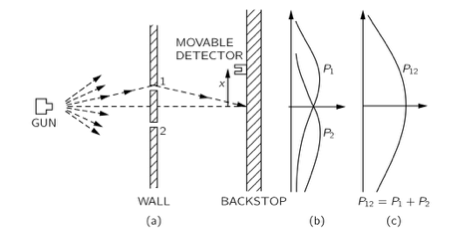
\includegraphics{gun_ds.png}
\end{figure}

  The gun shoots macroscopic bullets. We imagine the distance gun-screen to be large, implying that the bullets might arrive at different locations due to error, vibrations, wind etc. Therefore, we expect bullets to arrive as a beam.

  Most of the bullets will not reach the second wall, as they will remain stuck on the first one. However, the ones directed towards the holes will pass through. We expect to obtain a distribution of bullets for hole 1 and hole 2. If we shut down one hole 2, nothing will pass through it - leading to $p_1$ distribution. Conversely, if we shut down hole 1 we will observe $p_2$.
  
  Summarizing, we will find the following observations:
  \begin{enumerate}
      \item bullets arrive one-by-one, we can recognize the sound of each bullet impacting the screen (if sufficient resolution is available for the recording)
      \item $P(z)$, the probability of a bullet reaching a point, can be obtained by plotting a histogram of the times a bullet has hit the point of interest. Through a statistical model we could then predict future locations. 
       \item considering the experiment with one of the holes shut, a Gaussian like probability of detection $P_1$ can be seen such that $\mu$ is directly perpendicular to the hole.
       \item ff both holes are open there is a ballistic behaviour and the resulting distribution of detection $P_{12}$ is the sum of the two deriving for each hole open by itself: $$P_{12} = P_1+P_2$$ (disjoint event).
  \end{enumerate}
    
  
    \subsubsection{Case 2 - macroscopic waves in a tank}
    Suppose that rather than having a screen, we have a tank of water with a wall with two holes. In this case, we have an instrument producing waves e.g. something touching water. Since the source is very far, waves will reach the wall as it as plane waves. We want to measure whether the waves manage to impact the second wall. From each of the holes, we will observe circular waves. We can repeat the previous procedure of shutting each hole at a time. The maximum intensity (square of max amplitude) will be observed at the hole. 

  When the wave arrives, it reaches different locations at the same time (delocalization), very differently from bullets.   A second difference is what we obtain when we let waves pass through both holes. It has alternating minima and maxima and it can be seen that $P_{12} \neq P_1+P_2$. In this case we obtain an interference pattern, as waves can sum and subtract in a non-trivial way (waves are complex objects).
    So, deriving from wave theory:

    $$A_1\rightarrow P_1 = |A_1|^2 = A_1^*A_1$$
      
    $$A_2\rightarrow P_2 = |A_2|^2 = A_2^*A_2$$

    \begin{align*}
      A_{12} = A_1+A_2\rightarrow A_{12} &= |A_1+A_2|^2=\\
                                         &=A_1^*A_1 + A_2^*A_2 + \underbrace{A_1^*A_2 + A_1A_2^*}_{\text{interference}}
    \end{align*}

    Unlike bullets, wave hit the entire screen and not at a precise time.
    So a wave-like behaviour with de localization can be seen.

    \subsubsection{Case 3 - cathode as an electron gun}
    Finally, let us have a cathode electron gun shooting electrons at a wall with very small holes - which need to be so small that the effect becomes evident. As before, we close one of the holes and the screen will record the arrival of electrons on the wall through a detector (device producing a small signal as soon as an electron arrives). If we place many detectors on the wall, we will retrieve when and where the electron has arrived. The electron signals arrive one at a time, as a "rain". If we open both holes, an interference pattern will be observed: $P_tot$ is not the sum of the single probabilities, implying that the two are not disjoint events 
Result: we observe either a particle-like behaviour (one hole closed) or a wave-like behaviour (both holes open).
    
   
    
    To verify whether the electron goes through both holes simultaneously, an apparatus that emits a signal if an electron travels nearby is put near the holes.
    Detection on the screen happens only if the signal is emitted.
    The two apparatuses never trigger a signal together, meaning that the electron travels through one of the holes like a particle.
    We can define $P_{A_1}$ as the probability that counts only events in which $A_1$ is triggered and $P_{A_2}$ the results of counting only events triggering $A_2$.
    By counting all the events, it can be seen that the resulting pattern is $P_{A_1}+P_{A_2}$.
    In the case in which $P_{A_1+A_2} = P_{A_1} + P_{A_2}$, delocalization is lost and the electron assumes ballistic behaviour.
    Summarizing, measurement affects the nature of the electron and can change the state of the system.
When we try to measure where the particle goes, we observe a ballistic behaviour. Conversely, if we do not impose any measurement, we will obtain an interference pattern. The result depends on the kind of behaviour we are trying to detect. 

Example: suppose that we are blind. We can detect a ball by throwing something smaller at it e.g. pen cap. If instead we throw a pen cap towards with another pen cap, we will have a collision and both objects will end up in a different location. The act of measuring has changed the system! 
Throwing photons at electrons perturbes the system, as they are comparable in size.

    \subsubsection{Conclusions}
    The notion of trajectory loses significance for microscopic particles.
    This is quantified by Heisemberg's uncertainty principle:

    $$\underbrace{\Delta p}_{\text{Uncertainty on }p}\ \underbrace{\Delta q }_{\text{Uncertainty on }q} \ge \frac{\hbar}{2}$$

    It is impossible to simultaneously measure with arbitrary accuracy the position and the velocity of a microscopic particle.

\section{The photoelectric effect}
By considering the classical theory of the hydrogen atom and ignoring that energy loss through electromagnetic radiation would be unstable, this model can transfer any amount of energy to the electron by shining light on it.
In classical electromagnetism, the energy of radiation comes from the intensity of the electromagnetic wave.
It would be expected that, irregardless of the frequency or wave-length, the amount of electron extracted would scale with the intensity of the electromagnetic wave.

  \subsection{Experimental findings}
  Electrons are extracted only if the light has a $\nu > \nu_{\min}$ or $\lambda<\lambda_{\max}$.
  If $\nu>\nu_{\min}$, the amount of electrons scale with the intensity.

  \subsection{Conclusions}
  This experiment determined that the energy transfer depends on the frequency $\nu$ of the electromagnetic radiation.
  Moreover, electrons can only acquire certain quanta of energy.
  This led to the introduction of two pivotal concepts of modern physics.

    \subsubsection{Energy quantization}
    The amount of energy transfer to a bound system cannot be arbitrary small.

    \subsubsection{Photons}
    Light is made by the photon particle which carries energy $E = \hbar\nu$, where $\omega = 2\pi\nu$ and $\hbar = \frac{h}{2\pi}$, so:

    $$E = \hbar\omega$$

    Photons, like electrons, share wave-like and particle-like properties.
    Therefore, electrons can be considered as waves of matter and photons as particles of light.

\section{Quantization and atomic spectra}

  \subsection{Experiment}
  A beam of light goes through an atom and a prism.
  The prism splits the frequencies and those frequencies are collected on a screen.

  \subsection{Finding}
  By performing this experiment, it has been found that only certain frequencies can be absorbed by the atoms.

  \subsection{Conclusion}
  Only certain excitation energies are permitted and those form a characteristic signature of atoms:

  $$\hbar\omega = E_n-E_m$$

  Because of this finding, classical mechanics can be seen as a non-fundamental theory: it perfectly describes observations in some limited range of length, mass, temperature.
  Any more fundamental theory must contain classical mechanics as an approximation in the macroscopic regime, according to the correspondence principle.

\section{Stern Gerlach experiment}

  \subsection{Experiment}
  An electron beam shoots electrons with different momenta $\vec{\mu}$ through an inhomogeneous magnetic field $SG$.
  Behind this there is a screen that detects those electron. If we shut off the magnetic field, the electrons will not interact with anything and we will obtain a high peak. When we activate a magnetic field, there will be some electrons with magnetic moment aligned with velocity and basically left unchanged, while others will be deflected either up or down. We expect to see a wider distribution as a result.

  \subsection{Finding}
  Classically, the electrons are expected to be bended by $SG$ more or less depending on the orientation of $\vec{\mu}$, with an expected density shaped like a Gaussian with $\mu$ at the middle.
  Since $\hat{z}$ has been selected by $SG_1$, $SG_3$, it would be expected to find only $\mu_z = + \mu_0$. Instead, the final beam contains $\mu_z =\pm \mu_0$.

In real experiments what we see are two narrow peaks; the position of the peaks is compatible with a scenario in which all particles are completely aligned or completely unti-alinged with the z-axis. Somehow, the z component of the magnetic moment is QUANTIZED. It can only take maximum or negative maximum values. Other atoms provide different shapes e.g. up, down, zero. But let’s stick to the case in which we observe two peaks.
Suppose that now we insert a second device aligned to the x-axis. This time we are measuring the x-component of the magnetic field. Not only the z component is quantised, but also the x and y components.
\begin{enumerate}
  \item select z component
  \item filter positive z component
  \item select x component
  \item filter positive z component
  \item measure z component
 \end{enumerate}
We already measured the z component, so we expect x to be deflected in a single direction. Surprisingly, x will deflect to both positive and negative with equal probability. 

  \subsection{Conclusion}
  The act of measuring $\mu_x$ completely destroys the information about the state of $\mu_z$.
  According to the uncertainty principle, $\mu_x$ and $\mu_z$ cannot be simultaneously determined.
  Instead, we only find two possible orientations of the magnetic moment, that is in fact quantizied.
  Considering three $SGs$ in series with different orientations: $\hat{z}\rightarrow\hat{x}\rightarrow\hat{z}$:
  The first selects $\hat{\mu}_z = +\mu_0$ and the second $\hat{\mu}_x = +\mu_0$.

\section{Finding the Schr\"oedinger equation}
Particle propagation is not ballistic:

$$P_{12} \neq P_1 + P_2$$

Probability $P(2)$ displayed interference pattern.
Interference pattern naturally arises when taking squared modules of complex amplitudes:

\begin{align*}
  I_{12} &= |A_1 + A_2|^2=\\
         &=(A_1 + A_2)(A_1^*+A_2^*)^*=\\
         &=(A_1A_1^*+\underbrace{A_1A_2^*+A_2A_1^*}_{\text{interference pattern+}}A_2A_2^*)
\end{align*}


Considering $E=n\nu$ a wave function for the electron, a propagating wave can be written as:

$$f(x,t) = f_>(x-vt)+f_<(x+vt)$$

And:

\begin{align*}
  \biggl(\frac{1}{v^2}\frac{\partial {^2}}{\partial {t^2}}-\frac{\partial {^2}}{\partial {x^2}}\biggr)\begin{cases}f_>(x+vt)\\f_<(x-vt)\end{cases} &= 0\\
  \frac{1}{v^2}\frac{\partial {}}{\partial {t}}\biggl(\frac{\partial {}}{\partial {t}}f_>(x-vt)\biggr)&-\frac{\partial {}}{\partial {x}}\biggl(\frac{\partial {}}{\partial {x}}f_>(x+vt)\biggr)=\\
  -\frac{1}{v}\frac{\partial {}}{\partial {t}}[f_>'(x-vt)]&=f''_>(x-vt)\\
  f_>''(x-vt) &=f''_>(x-vt)
\end{align*}

Now an electron is assumed to propagate as a wave $\psi(x.t)$ for which: $|\psi(x,t)|^2 = P(x,t)$.
Trying to apply a photon wave to the electron:

$$\psi(x,t) = A_oe^{i(vt-kx)} = \cos(vt-kx) + i\sin(vt - kx)$$

Considering that both the real and imaginary part oscillate:

\begin{align*}
  \begin{cases}\frac{\partial {^2}}{\partial {t^2}}A_0e^{i(vt-kx)} = A_0(-v^2e^{i(vt-kx)})\\\frac{\partial {^2}}{\partial {x^2}}A_0e^{i(vt-kx)} = A_0(-k^2e^{i(vt-kx)})\end{cases}&\rightarrow \frac{1}{\nu^2}\biggl[-A_0v^2e^{i(vt-kx)}+A_0k^2e^{i(vt-kx)}\biggr] = 0\\
                                                                                                                                                                                  &\Rightarrow \nu = v^2k^2\text{ frequency or velocity of propagation}
\end{align*}

From this it can be seen that $E=\nu h\propto v$, but because of the mass of the electron it should be that $E\propto v^2$.
So the Schr\"oedinger equation is a modified wave equation to accomodate this:

$$ia \frac{\partial {}}{\partial {t}}\psi=-d \frac{\partial {^2}}{\partial {x^2}}\psi(x,t)$$

  \subsection{Free particle Schr\"oedinger equation}
  In this equation, particle interactions and potential energy are not considered:

  $$i\hbar \frac{\partial {}}{\partial {t}}\psi(x,t) = \frac{\hbar^2}{2m}\frac{\partial {^2}}{\partial {x^2}}\psi(x,t)$$

  \subsection{Complete Schr\"oedinger equation}
  By allowing the electron to react, we can introduce the operator $H$ - which is composed by kinetic energy and potential energy component (as the classical Hamiltonian). Based on this, we can refer to the operator as Quantum Hamiltonian.
  It can be seen how the potential energy is more important than the force:

  $$i\hbar \frac{\partial {}}{\partial {t}}\psi(x,t) = \overbrace{\biggl[-\underbrace{\frac{\hbar^2}{2m}\frac{\hat{\partial} {^2}}{\partial {x^2}}}_{\text{kinetic energy operator}}+\underbrace{\hat{U}(x)}_{\text{quantum energy operator}}\biggr]}^{\text{Quantum Hamiltonian}}\psi(x,t) = \hat{H}\psi(x,t)$$
  This is a partial differential equation (PDE) describing the evolution over time of the wavefunction. Uncertainty is reflected by the fact that we do not talk about a space trajectory, the interpretation is stochastic (as the wavefunction is a probability). Therefore, QM is not about the nature itself, but rather about predicting the outcomes of experiments on nature. The entire foundation of QM is computing the probability for an outcome of an experiment. 

    \chapter{Waves of matter}

\section{The Schr\"odinger equation}
Physical laws can never be demonstrated, but only inferred from experiments and then verified or falsified by other ones.


  \subsection{Double-slit experiment}
  The propagation of the electrons in the double-slit experiment has wave-like properties.
  The probability of an electron being detected in certain points of the screen is described by complex-wave amplitudes, which are functions of $x$ and $t$. Being $A(x,y)$ a wave, its intensity:

  $$Intensity(x,t) = A^*(x,t)\cdot A(x,t)$$

  The state of the electron in the beams is assumed to be described by a complex amplitude called the wave-function:

  \begin{align*}
    \psi(x,t) &\rightarrow Prob(x,t)\\
              &=\psi^*(x,t)\psi(x,t)\\
              &\equiv |\psi(x,t)|^2
  \end{align*}

  \subsection{Main assumption}
  Electrons behave exactly like photons: they both have a dual particle and wave nature.
  As a consequence, we can assume that for an electron the energy is proportional to frequency:

  $$E = \hbar\omega = h\nu = \frac{p^2}{2m}$$

  Protons propagate according to a wave equation:

  $$\biggl(\underbrace{\frac{1}{c^2}}_{\text{speed of light}}\frac{\partial^2{}}{\partial{t^2}} - \nabla^2\biggr)\underbrace{A}_{\text{Maxwell equation}} = 0$$

  There is a need to find if the same equation describes the propagation of a massive particle like the electron.
  Let the electron wave particle be:

  $$\psi(x,t) = Ae^{\frac{i}{\hbar}(Et -px)}$$


  Then: $\frac{\partial^2{}}{\partial{t^2}}\psi = \omega^2\psi$ and $\frac{partial^2}{\partial x^2}\psi = p^2\psi$.
  So it is obtained that:

  $${p^2}\propto\underbrace{\omega^2}_{\propto E^2}$$

  Then $E = cons|p|$.
  This is true for light, but it is false for massive particles. The correspondence principle implies that:

  $$E = \frac{p^2}{2m}\rightarrow E\propto p^2$$

  And not just to $|p|$.

  \subsection{Defining the Schr\"oedinger equation}
  There is a need to use a different wave equation with respect to the photon's one.
  Noticing that $E^2\propto p^2$ follows from having two time derivatives, we can try a first time derivative to obtain $E\propto p^2$.
  Then the equation to solve becomes:

  $$\biggl(iC_1\frac{\partial}{\partial t} C_2\frac{\partial^2}{\partial x^2}\biggr)\psi = 0$$

  \begin{align*}
    \begin{cases}\frac{\partial\psi}{\partial t} = A\frac{i}{\hbar}E\psi(x,t)\\\frac{\partial^2\psi}{\partial x^2} = A\frac{-1}{\hbar^2}p^2\psi(x,t)\end{cases}\\
    \biggl(C_1\frac{\partial}{\partial t} - C_2\frac{\partial^2}{\partial x^2}\biggr)\psi(x,t) &=0\\
    \biggl(C_1\frac{i}{\hbar}E-C_2\bigl(-\frac{1}{\hbar^2}p^2\bigr)\biggr)\psi(x,t) &= 0\\
    \biggl(C_1\frac{i}{\hbar}E-C_2\bigl(-\frac{1}{\hbar^2}p^2\bigr)\biggr) &= 0\\
  \end{align*}

  Now, considering $\frac{C_1}{C_2}=R\rightarrow \hbar^2$:

  $$\begin{cases} i\underbrace{\hbar\frac{\partial}{\partial t}\psi}_{\text{kinetic energy}}-\frac{\hbar^2}{2m}\frac{\partial^2}{\partial x^2}\psi = 0\\E =\frac{p^2}{2m}\\E = \hbar\omega\end{cases}$$

  Now:

  $$\hbar\omega = E \propto p^2$$
  Recall that $\hbar$ is the Dirac's constant, obtained by the following formula: $\hbar=frac{h}{2\pi}$, where $h$ is the Planck's constant.
  
  For a free electron, $H$ equals the kinetic energy and is approximately the Hamiltonian.
  For an interacting electron:

  $$H_0 \rightarrow H_0 + \underbrace{V(\vec{r})}_{\text{potential energy}} = H$$

  Finally, the Schr\"oedinger equation is:

  $$i\hbar \frac{\partial {}}{\partial {t}}\psi(\vec{r},t) = \biggl(-\frac{\hbar^2}{2m}\nabla^2+V(\vec{r})\biggr)\psi(x,t)$$

    \subsubsection{Quantum Hamiltonian}
    The quantum Hamiltonian can be defined as:

    $$\hat{H} \equiv -\frac{\hbar^2}{2m}\frac{\partial^2}{\partial x}+U(x)$$

    Comparing it with a classical Hamiltonian, it can be seen that $\frac{p^2}{2m}\xrightarrow[]{\text{quantization}} - \frac{\hbar^2}{2m}\frac{\partial^2}{\partial x^2}\Rightarrow p^2\rightarrow \hbar^2\frac{\partial^2}{\partial x^2}$.
    Then, due to the fact that the forward propagating wave has a positive momentum, $\hat{p}\rightarrow i\hbar\frac{\partial}{\partial x}$.
    The same happens in three dimensions, where:

    $$i\hbar\frac{\partial }{\partial x}\psi(\vec{x}, t) = \biggl(-\frac{\hbar^2}{2m}\nabla^2+U(\vec{x})\biggr)\psi(\vec{x},t)$$

    The Schr\"oedinger equation is then recast as:

    $$i\hbar \frac{\partial {}}{\partial {t}}\psi(\vec{r},t) = \hat{H} \psi(\vec{r},t)$$

    To solve this equation there is a need to solve a partial differential equation that defines the state of a system.
    The operators are:

    $$\hat{H} = \biggl(-\frac{\hbar^2}{2m}\nabla^2+U(\vec{r})\biggr)$$
    
    $\hat{H}$ operates on the function $\psi$, giving as a result a new function $\psi'$.
    Note that $$\hat{H}(a\psi_1(x,t)+b\psi_2(x,t)=a\hat{H}\psi_1+b\hat{H}\psi_2$$.
    $\hat{H}$ is a linear operator, acting on a space of function (Hilbert space) and giving as a result a new function through a linear transformation. 
    
    $$\nabla^2 = \biggl(\frac{\partial^2}{\partial x^2} +\frac{\partial^2}{\partial y^2} + \frac{\partial^2}{\partial z^2}\biggr)$$

\section{Stationary Schr\"oedinger equation}
Assuming that the system conserves mechanical energy:

$$H(p,q, \bcancel{t}) = \frac{p^2}{2m}+U(q,\bcancel{t})$$

Considering the plane wave:

$$\psi(\vec{r}, t) = \phi(\vec{r}) e^{-i \frac{E}{\hbar}t}$$
In this case, $\psi$ is factorized into two terms - which we can call $\phi$ and $\xi$.

By formulating a guess for the form of the solution and plugging it into the Schr\"oedinger equation:

$$E\phi e^{-i \frac{i}{\hbar}(Et)} = He^{-\frac{i}{\hbar}Et}\phi$$

Which gives:

$$\hat{H}\phi(\vec{r}) = E\phi(\vec{r})$$

Where $E$ is unknown.

This is an eigen problem: given $\hat{H}$, a function $\psi(\vec{r})$ has to be found such that $\hat{H}\psi(\vec{r})$ is a function proportional to $\psi(\vec{r})$ through some constant $E$.
In other words, the energy of a quantum system is an eigenvalue of the quantum Hamiltonian operator.
Energy quantization is obtained and:

$$E = \underbrace{E_0}_{\text{ground state energy}} < \underbrace{E_1 < \cdots < E_n}_{\text{excited state energies}}$$

And:

\begin{align*}
  \hat{H}\psi(\vec{r}) &= E_0\psi_0(\vec{r})\\
  \hat{H}\psi(\vec{r}) &= E_1\psi_1(\vec{r})\\
                       &\vdots\\
  \hat{H}\psi(\vec{r}) &= E_n\psi_n(\vec{r})\\
\end{align*}

\section{Ground state of the quantum harmonic oscillator}
The quantum Hamiltonian for the quantum harmonic oscillator is:

$$\hat{H} = - \frac{\hbar^2}{2m}\frac{d{^2}}{d{x^2}} +\frac{1}{2}m\omega^2 x^2$$

The solution for the ground state should be in the form $\hat{H}\psi_0 = E$.

  \subsection{Form of the ground state}
  The ground state will be in the form:

  $$\psi(x) = \mathcal{N}e^{-\frac{\alpha x^2}{4}}$$

  So:

  \begin{align*}
    -\frac{\hbar^2}{2m}\frac{d{^2}}{d{x^2}}\phi_0 &= -\frac{\hbar^2}{2m}\mathcal{N}\frac{d{}}{d{x}}\biggl[-\frac{\alpha}{2}xe^{-\frac{\alpha x^2}{4}}\biggr]=\\
                                                  &= -\frac{\hbar^2}{2m}\biggl[-\frac{\alpha}{2}e^{-\frac{\alpha x^2}{4}}+\frac{\alpha^2}{4}x^2e^{-\frac{\alpha x^2}{4}}\biggr]\mathcal{N}
  \end{align*}

  So:

  \begin{align*}
    \hat{H}\phi_0 &= -\frac{\hbar^2}{2m}\frac{d{^2}}{d{x^2}}\phi_0 + \frac{1}{2}m\omega^2x^2\phi_0=\\
                  &= \frac{\alpha}{4}\frac{\hbar^2}{m}\phi_0 -\frac{\hbar^2\alpha^2}{8m}x^2\phi_0 + \frac{1}{2}m\omega^2x^2\phi_0
  \end{align*}

  For $\phi_0$ to be an eigenstate $\hat{H}\psi_0 = const\cdot\psi_0$, so the dependence on $x^2$ must be cancelled:

  $$-\frac{\hbar^2}{8m}\alpha^2\bcancel{x^2}\bcancel{\phi_0} + \frac{1}{2}m\omega^2\bcancel{x^2}\bcancel{\psi_0} = 0$$

  From this:

  $$\alpha^2 = \frac{4m^2\omega^2}{\hbar^2}\Rightarrow\alpha=\frac{2m\omega}{\hbar}$$

  So the solution is:

  $$\phi_0(x) = \mathcal{N}e^{-\frac{2m\omega}{\hbar}x^2}$$

  \subsection{Solution of the ground state of the quantum mechanic oscillator}
  The one dimensional quantum mechanic oscillator is the most used model:

  $$H = -\frac{\hbar^2}{2m}\frac{\partial^2}{\partial x^2} + \frac{1}{2}m\omega^2x^2$$

  A wave function for a one particle system contains zero nodes for the ground state.
  It is expected that the ground state is different from zero and we assume a Gaussian for a solution:

  $$\phi_0(x) = \mathcal{N} e^{\alpha x^2}$$

  The objective is to compute $\hat{H}\phi_0 = n\phi_0(x)$:

  \begin{align*}
    \hat{H}\phi_0 &= -\frac{\hbar^2}{2m}\frac{\partial^2}{\partial x^2}(\mathcal{N}e^{-\alpha x^2}) = -\frac{\hbar^2}{2m}\frac{\partial}{\partial x}(-2\alpha x e^{-\alpha x^2})\mathcal{N}=\\
                  &=-\frac{\hbar^2}{2m}(-2\alpha e^{-\alpha x^2}+4\alpha xe^{-\alpha x^2})\mathcal{N}=\\
                  &= \frac{\hbar^2}{\bcancel{2}m}\bcancel{2}\alpha\phi_0 -\frac{\hbar^2}{2m}4\alpha^2 x^2\phi_0\\
    \hat{H}\phi_0 &= \underbrace{\frac{\hbar^2}{m}\alpha\phi_0(x)}_{n\phi_0(x)} + \underbrace{\biggl(\frac{1}{2}m\omega^2-\frac{\hbar^2}{m}\alpha^2\biggr)x^2\phi_0(x)}_{\text{depends on }x^2}
  \end{align*}

  The solutions are found for values of $\alpha$ that set to $0$ the part dependent on $x^2$:

  \begin{align*}
    \frac{1}{2}m\omega^2 -\frac{\hbar^2}{m}2\alpha^2 &= 0\\
    \alpha &= \frac{m\omega}{2\hbar}
  \end{align*}

  Therefore the Gaussian is a good solution:

  $$\phi_0(x) = \mathcal{N}e^{-\frac{m\omega^2x}{2\hbar}}$$

    \subsubsection{Normalization evaluation}
    Consider that $\frac{1}{\sigma^2} = \frac{m\omega}{\hbar} \rightarrow \sigma^2 = \frac{\hbar}{2m\omega}\rightarrow \sigma = \sqrt{\frac{\hbar}{2m\omega}}$.
    Then consider:

    $$\mathcal{N}\int_{-\infty}^\infty e^{-\frac{m\omega x^2}{\hbar}}$$

    And solve the Gaussian integral:

    $$\int e^{-\sigma x^2} = \sqrt{2\pi}\sigma$$

    Then:

    \begin{align*}
      \mathcal{N}^2 &= \frac{1}{\int|\phi_0|^2dx} = \frac{1}{(2\pi\sigma)^{\frac{1}{2}}} = \frac{1}{(2\pi\sqrt{\frac{\hbar}{2m\omega}})^\frac{1}{2}}\\
      \mathcal{N} &= \frac{1}{(2\pi\sqrt{\frac{\hbar}{2m\omega}})^{\frac{1}{4}}}
    \end{align*}

    \subsubsection{Compute the average value of kinetic and potential energy}
    Due to the fact that operations are stochastic, the outcome cannot be predicted. We can only compute the probability or the average values.
    Let $\langle U\rangle $ be the average value of the potential energy, then:

    \begin{align*}
      \langle U\rangle  &= \int P_0(x)U(x)dx = \frac{\int dx e^{-\frac{m\omega x^2}{\hbar}}\frac{1}{2}m\omega^2x^2}{\int dx e^{-\frac{m\omega x^2}{\hbar}}} =\\
          &= \frac{1}{2}m\omega^2\underbrace{\langle x^2\rangle }_{\text{variance }\sigma^2} = \frac{1}{2}\bcancel{m}\omega^{\bcancel{2}}\frac{\hbar^2}{2\bcancel{m}\bcancel{\omega}}=\\
          &=\frac{1}{4}\hbar\omega
    \end{align*}

    So considering $E_0 = \frac{1}{2}\hbar\omega$, the energy remains the same, but the potential energy changes stochastically. Then:

    $$E_0 = \langle U\rangle  + \langle T\rangle $$

    In order to compute the kinetic energy, we need to consider that in quantum mechanics anything that can be measured except time is an observable.
    So, starting with classical mechanics, the observable $o(p,q)$ momentum and position, and after quantization and using the position representation:

    \begin{align*}
      O(\underbrace{\hat{p}}_{-i\hbar\vec{\nabla}},\underbrace{\hat{q}}_{\vec{q}}) &\rightarrow \hat{O}\\
      T = \frac{p^2}{2m}&\rightarrow \hat{T} = \frac{\hat{p}^2}{2m} = \frac{(-i\hbar\nabla)^2}{2m} = -\frac{\hbar^2\nabla^2}{2m}\\
      U(q)&\rightarrow \hat{U}
    \end{align*}

    Now considering the orbital angular momentum $\vec{L} =\vec{r}\cdot\vec{p}$:

    $$\begin{vmatrix}i&j&k\\x&y&z\\P_x&P_y&P_z\end{vmatrix}$$

    Then:

    $$L_z = xP_y - yP_x\xrightarrow[]{\text{quantization}}x\biggl(-i\hbar\frac{\partial}{\partial y}\biggr) - y\biggl(-i\hbar\frac{\partial}{\partial x}\biggr)$$

    Now considering $\langle \phi|O|\phi\rangle$ that specifies the state and that is equivalent to $\langle O\rangle$, where:

    $$\langle O\rangle = \frac{\int dx \phi^*(x)(O(x)\cdot\phi(x))}{\int dx\phi^*(x)\phi(x)}$$

    Then:

    \begin{align*}
      \langle\phi|\hat{T}|\phi\rangle &=\frac{\int dx\phi^*(x)(-\frac{\hbar^2}{2m}\frac{\partial^2}{\partial x^2}\phi(x))}{\int dx |\phi(x)|^2 = \frac{1}{4}\hbar^2}=\\
                                      &=e^{-\alpha x^2}\frac{\partial^2}{\partial x^2}e^{-\alpha x^2} = e^{-\alpha x^2}\frac{\partial}{\partial x}(-2\alpha xe^{-\alpha x^2}) =\\
                                      &=e^{-\alpha x^2}(-2\sigma w^{-\alpha x^2}+4\alpha^2x^2e^{-\alpha x^2})= \\
                                      &=-2\alpha|\phi|^2 = 4\alpha^2 x^2|\phi|^2
    \end{align*}

    And so:

    $$\langle\phi|\hat{T}|\phi\rangle = \frac{-\frac{\hbar^2}{2m}\int |\phi(x)|^2dx}{\int|\phi(x)|^2}2\alpha= - \frac{\hbar^2}{2m}4\alpha^2\frac{\int dx|\psi|^2x^2}{\int dx|\psi|^2}$$


\section{Quantum particle in a one dimensional infinite square well}
We previously discussed at the classical level that a physical system can be bound or unbound. In quantum physics, a bound state is a quantum state of a particle subject to a potential such that the particle has a tendency to remain localized in one or more regions of space. Ultimately, matter and life exist because of bound systems, which allow the presence of macro structures.  
While trying to solve a bound system problem, we will require a toy model - a model deliberately too simple to be realistic, which is not meant to predict the outcome of an experiment, but rather to understand the qualitative nature of the object under study.
While implementing a toy model, if the scale where a detail occurs is very small compared with the size of the box, its effect can be neglected. As a consequence, everything which occurs within the box is idealized, allowing us to solve the problem. It's all a matter of scale e.g. $\lambda$ is the scale for details, $L$ the size of the physical system, $\eta$ the energy we are interested in, $E$ the unbounding energy. If the ratio $\frac{\lambda}{L}<<<1$ and $\frac{\eta}{E}<<<1$ , we can neglect the detail.

For the case of a quantum particle in a one dimensional infinite square well, we will consider a particle constrained in a trap where interactions are so strong that it cannot escape and with two confining directions much narrower than the third. We can consider a box with size $L/2$ and $-L/2$ and find the eigenvalues and eigenvectors for the SE in this specific condition. 
This can be modelled with a one dimensional confining potential:

$$U(x) = \begin{cases} 0, &-\frac{L}{2}<x<\frac{L}{2}\\\infty &|x|>\frac{L}{2}\end{cases}$$

Inside the box $U=0$, so the Schr\"oedinger equation is:

$$-\frac{\hbar^2}{2m}\frac{d{^2}}{d{x^2}}\psi(x) = E\psi(x)$$

Mathematically this looks like the Newton's equation for the harmonic oscillator:

$$+m \frac{d{^2}}{d{t^2}}x(t) = -kx(t)$$

Where $x\rightarrow t$ and $\psi\rightarrow x$.
However, the constraints are different. Instead of the classical initial values $x(0) = x_0$ and $\frac{d{}}{d{t}}x|_{t=0} = 0$, there is a boundary value $\psi\biggl(\pm \frac{L}{2}\biggr) = 0$.

  \subsection{Solution}
  Given the mathematical similarity between the two equations, the general structure of the solution should be:

  $$\psi(x) = \begin{cases}A_1\cos k_1 x \\A_2\sin k_2x\end{cases}$$

  Where $A_1,A_2,k_1, k_2$ need to be fixed.

    \subsubsection{Option 1}
    $A_1\cos\biggl(k_1 \frac{L}{2}\biggr) = 0$, then:

    \begin{align*}
      k_1 \frac{L}{2} &=\pm \frac{\pi}{2}\pm n\pi\Rightarrow\\
      \Rightarrow k_1^{(n)} &=\pm \frac{\pi}{L},\pm \frac{3\pi}{L},\dots =\\
                            &= \pm 2(n-1)\frac{\pi}{L}\qquad n = \mathbb{N}
    \end{align*}

    For this option, the possible quantized energy levels are:

    $$E^{(n)} = \frac{\hbar^2}{2m}\frac{\pi^2}{L^2}(2n-1)^2$$

    \subsubsection{Option 2}
    $A_1\sin\biggl(k_2 \frac{L}{2}\biggr) = 0$, then:

    \begin{align*}
      k_2 \frac{L}{2} &=\pm \pi\pm n\pi\Rightarrow\\
      \Rightarrow k_2^{(n)} &=\pm \frac{2\pi}{L},\pm \frac{4\pi}{L},\dots =\\
                            &= \pm 2n\frac{\pi}{L}\qquad n = \mathbb{N}
    \end{align*}

    For this option, the possible quantized energy levels are:

    $$E^{(n)} = \frac{\hbar^2}{2m}\frac{\pi^2}{L^2}(2n)^2$$

    \subsubsection{$A_1$ and $A_2$}
    $A_1$ and $A_2$ can be determined by applying the normalization conditions.
    The probability of finding the particle somewhere in the box is one, so:

    \begin{align*}
      \int_{-\frac{L}{2}}^{\frac{L}{2}} dx|\psi(x)|^2 = 1\\
      1 = \int_{-\frac{L}{2}}^{\frac{L}{2}} dx\begin{cases}A_1^2\cos^2k_1x\\A_2^2\sin^2 k_2x\end{cases}\Rightarrow\begin{cases}A_1 = \\A_2 = \end{cases}
    \end{align*}

    \subsubsection{Summary}
    Summarizing the results:

      \paragraph{Energy spectrum}

      $$E_n = \frac{\hbar^2}{2m}\frac{\pi^2}{L^2}\mathcal{L}^2$$

      \paragraph{Energy eigenstates}
      The energy eigenstates of the stationary wave-functions are:

      $$\psi_m(x) = \begin{cases}A_1\cos k_1 x & n\ odd\\ A_2\sin k_2 x & n\ een\end{cases}$$
      

  \subsection{Discussion}

    \subsubsection{Quantized momenta}
    From the quantized energy:

    $$E_n = \frac{1}{2m}\biggl(\underbrace{\frac{\pi^2\hbar^2}{L_2}m^2}_{=p_m^2}\biggr)$$

    So the quantized momenta is $p_m = \pm \frac{\pi\hbar}{L}m$.
    For each value of $v$ p=mv and Ep=p^2/2m, infititely many kinetic energies. In phase space we keep p0 constant, then reflection occurs to -p0, until a position oon the other wall is reached. Projections look like squares; if we start with a lower momentum, we are going to obtain a smaller rectangle. In principle we can choose any value for p, no restrictions. This is not what happens with quantum particles, where we only have some allowed $p_n=k_n\hbar$ momenta.
    
    \subsubsection{Lowest energy state}
    In classical mechanics, the lowest energy state is $p = 0\Rightarrow E = 0$. 
    Differently, in quantum mechanics the lowest energy level is:

    $$E_1 = \frac{\hbar^2}{2m}\biggl(\frac{\pi}{L}\biggr)^2 > 0$$

    Recalling that $E_1 = \frac{p_1^2}{2m}$, it is inferred that:

    $$p_1 = \pm \frac{\hbar\pi}{L}\neq 0$$

    $p_1$ can point in $+$ or $-$ direction with equal probability, so the quantum uncertainty is $\Delta p =\frac{2\hbar\pi}{L}$.
    On the other hand, $\Delta p \sim L$, so there is quantum delocalization for $\psi_1(x)$.
    However in the classical ground state:

    $$T = \frac{p^2}{2m = 0}\Rightarrow p = 0\Rightarrow \Delta p = 0$$

    But $\Delta q = b$, hence there is a violation of the uncertainty principle:

    $$\Delta q\Delta p = 0$$.

    \subsubsection{Correspondence principle}
    By considering that for $L\rightarrow\infty$ and $m\rightarrow\infty$ $E_0 = 0$, there is no uncertainty in classical mechanics. In addition, $E_{n+1}-E_n \rightarrow 0$, so there is no quantization.
    As a consequence, classical mechanics is contained in quantum mechanics in the macroscopic limit, for large size and heavy masses.

    \subsubsection{Excited states}
    The wave function of the n-th excited state has $N$ nodes, a general result that holds for any quantum system.

\section{Two dimensional square well}
Consider a quantum particle in a two dimensional square well with dimensions $L_1$ and $L_2$.
%insert image%
Then:

$$\hat{H} = -\frac{\hbar^2}{2m}\frac{\partial {^2}}{\partial {x^2}}-\frac{\hbar^2}{2m}\frac{\partial {^2}}{\partial {y^2}}$$

Any $H$ can be separated as: $H(x,y) = H_1(x) + H_2(y)$.
Anytime the Hamiltonian factorizes, i.e. $\hat{H}=\sum_i{\hat{h}_i}$, the solution of the SE can be written as the product of two wavefunctions $\phi(x,y)=phi_1(x)\phi_2(y)$. The corresponding energy will be obtained by summing the two energies $E=E_1+E_2$. By applying this property, we can write the solution to the Hamiltonian for our problem.
  
  \subsection{Solution}
  The solution is:

  $$\begin{cases}\phi(x,y) = \phi_1(x)\phi_2(y)\\H\phi=(E_1+E_2)\phi\end{cases}$$

  Where $H_1\phi_1 = E_1\phi_1$  and $H_2\phi_2 = E_2\phi_2$
  So:

  \begin{align*}
    (H_1 + H_2)\phi_1(x)\phi_2(y) &= H_1\phi_1(x)\phi_2(y) + H_2\phi_1(x)\phi_2(y)=\\
                                  &= \phi_2(y)\hat{H}_1\phi_1(x)+\phi_1(x0+\phi)1(x)H_2\phi_2(y)=\\
                                  &= \phi_2 E_1\phi_1 + \phi_1E_2\phi_2=\\
                                  &=(E_1+E_2)\phi_1\phi_2
  \end{align*}

  So:

  $$\phi_{n,m}(x,y) = \underbrace{\phi_n(x)}_{\text{solution of the 1D problem}}\phi_m(y)$$

  And $E_{n,m} = E_n^x+E_m^y = -\frac{\hbar^2}{2m}\pi^2\biggl(\frac{n^2}{L_x^2}+\frac{m^2}{L_y^2}\biggr)$.
  Then the ground state is $E_{11} = E_1^x+E_1^y$ and the system is doubly degenerative in opposite directions:

  $$E_{12} + E_1^x+E_2^y + E_{21} = E_2^x+E_1^y$$

\section{Lattice discretization}
Lattice discretization is a technique by which a numerical solution is obtained by exploiting the connection between operators and matrices.
A large but finite number of equally spaced possible position is used.
The possible positions are $x = x_{\min} + \Delta x$, where $\Delta x = \frac{x_{\max}-x_{\min}}{N}$.
The wave function is represented by a list $\psi(x) \rightarrow(\psi_1,\dots, \psi_N)$.
Thus, the wave function becomes a vector and the Hamiltonian a matrix.

  \subsection{Discrete representation of the derivative}

  $$\frac{d{}}{d{x}}\psi(x) \rightarrow \frac{\psi_{i+1}-\psi_i}{\Delta x}$$

  $$\frac{d{^2}}{d{x^2}}\psi(x) \rightarrow \frac{\psi_{i+1}+\psi_{i-1}-2\psi_i}{\Delta x^2}$$

  Let the Kronecker delta be:

      $$\delta_{ij} =\begin{cases}1 &i=j\\0 &i\neq j\end{cases}\Rightarrow S_{ij} \rightarrow\begin{pmatrix}1 & 0 & \cdots\\\vdots & \ddots &\vdots \\0&\cdots & 1 \end{pmatrix}$$

  Now:

  $$-\frac{\hbar^2}{2m}\frac{d{^2}}{d{x^2}}\rightarrow T_{ij}=-\frac{\hbar^2}{2m\Delta x^2}(\delta_{ij+1}+\delta_{ij-1}-2\delta_{ij})$$

  Indeed:

  $$\sum\limits_{j}T_{ij}\psi_i = -\frac{\hbar^2}{2m}(\psi_{i+1}+\psi_{i-1}-2\psi_i)\frac{1}{\Delta x^2}$$

  Now $V(x) \rightarrow V_{ij} = V_i\delta_{ij}$, so:

  $$\sum\limits_{j}V_{ij}\psi_j = V_i\psi_i$$

  Finally:

  $$H_{ij} = T_{ij} + V_{ij}$$

  $$H_{ij} = \begin{pmatrix}\frac{\hbar^2}{m\Delta x^2} + V_1 & -\frac{\hbar^2}{2m\Delta x} & 0 & \cdots\\ -\frac{\hbar^2}{2m\Delta x^2} & \frac{\hbar^2}{m\Delta x^2}+V_2-\frac{\hbar^2}{2m \Delta x^2} & 0 & \cdots\\ 0 & -\frac{\hbar^2}{2m\Delta x^2} & \frac{\hbar^2}{m\Delta x^2}+V_3 - \frac{\hbar^2}{2m\Delta x^2} & \cdots\end{pmatrix}$$

  Solving the matrix eigenproblem $\sum\limits_i H_{ij}\psi_i = E_i\psi_i$ yields $\{E_i\}_{i=\{1,\dots,N\}}$ and $\{y_j\}_i$.
  The dimensionality grows with the number of mesh points $N$.
  The exact case is $N\rightarrow\infty$.
  Quantum mechanics is described by an infinite dimensional vector space called the Hilbert space.

\section{Time evolution operators}
Consider the time-dependent Schr\"oedinger equation:

$$i\hbar\frac{\partial}{\partial t}\psi(x,t) = \hat{H}\psi(x,t)$$

Where:

$$\psi(x,t) = e^{-\frac{i}{\hbar}\hat{H}(t-t_0)}\psi(x,t_0)$$

And the time-evolution operator:

$$U(t,t_0) = e^{-\frac{i}{\hbar}\hat{H}(t-t_0)}$$

If the argument of the Taylor expansion is too large, we will infinitely many operators - unless it is a special quantum mechanics operators such that it is the eigenvalues of the Hamiltonian.
Let $\vec{a}_k$ be an eigenvector, then:

$$e^{\hat{A}}\vec{a}_k = e^{a_k}\vec{a}_n$$

As a consequence, the time-evolution operator for the eigenvectors of the Hamiltonian can be easily evaluated.
If $\psi(x,t=t_0) = \phi_n(x)$, where $\hat{H}\phi_n(x) = E_n\phi_n(x)$, then:

$$\psi(x,t) = e^{-\frac{i}{\hbar}(t-t_0)E_n}\phi_n(x)$$

And:

$$P(x,t) = |\psi(x,t)|^2 = |e^{-\frac{i}{\hbar}(t-t_0)E_n}|^2|\phi_n(x)|^2$$

If it has a pure phase: $|e^{ia}|^2 = e^{ia}(e^{ia})^* = e^{i(a-a)} = 1$, then:

$$P(x,t) = |\phi_n(x)|^2 = P(x,t)0$$

And it is the same as the initial time.

    \input{chapters/04_quantum_mechanics}

  \part{Quantum chemistry}

    \input{chapters/05_approximation_methods}
    \graphicspath{{chapters/06/}}
\chapter{Atomic physics}
\section{Quantum theory of the Hydrogen atom}
\subsection{Evaluation of conservation of energy}
In classical mechanics I can write
\[
E=\frac{1}{2}m\bigg(\frac{d}{dt}n\bigg)^2+\frac{L^2}{2mr^2}+U(r)
\]
that can be represented in quantum mechanics with the hamiltonian. The best evaluation of the hamiltonian for the quantum analysis of the hydrogen atom is obtained by using the \textbf{spherical coordinates}. Nabla in spherical coordinates $(r,\theta,\varphi)$ is hence written as:
\[
\nabla^2=\frac{1}{r^2}\frac{\partial^2}{\partial r^2}+\frac{1}{r^2}\cdot\bigg(\frac{\partial^2}{\partial \theta^2}+\frac{1}{\tan\theta}\frac{\partial}{\partial\theta}+\frac{1}{\sin\theta}\frac{\partial^2}{\partial\varphi^2}\bigg)
\]
The hamiltonian so becomes:
\[
\hat{H}=\frac{\hbar^2}{2mr^2}\frac{\partial^2}{\partial r^2}+\frac{\hbar^2}{2mr^2}\cdot\bigg(\frac{\partial^2}{\partial \theta^2}+\frac{1}{\tan\theta}\frac{\partial}{\partial\theta}+\frac{1}{\sin\theta}\frac{\partial^2}{\partial\varphi^2}\bigg)-\frac{e^2}{r}
\]
The first part is called \textbf{radial part} because it's $r$-dependent only, the other is the \textbf{angular part}.\\
Now I can consider the angular momentum in classical mechanics and quantum mechanics:
\[
\vec{L}=\vec{r}\times\vec{p}=\vec{r}\times(-i\vec{\nabla}\hbar)
\]
\[
\rightarrow \vec{\hat{L^2}}=\hat{L_x}\hat{L_x}+\hat{L_y}\hat{L_y}+\hat{L_z}\hat{L_z}
\]
This is corresponding to the angular part of the hamiltonian that can be rewritten with the inclusion of the angular momentum multiplied by $\hbar^2$.
\[
\hat{H}=\frac{\hbar^2}{2mr^2}\frac{\partial^2}{\partial r^2}+\frac{\hat{L^2}}{2mr^2}-\frac{e^2}{r}
\]
The fact that the angular momentum is not present in the radial part of the hamiltonian means that the two operators must commute $[\hat{H},\,\hat{L^2}]=0$ and they must also share the same eigenstates. It's also important to note that the invidual components of the angular momentum only commute with $\hat{L^2}$ but not with each other.\\
\[
\begin{cases}
[\hat{L_i},\,\hat{L_j}]\neq0 & i,j=1, 2, 3, ...\\
[\hat{L_i},\,\hat{L^2}]=0
\end{cases}
\]
\\
These are called \textbf{SPHERICAL HARMONICS}, they depend on two quantum numbers because they use two different operators and are only part of the angular part of the hamiltonian.\\
\[
\begin{cases}
\hat{L_z}Y(\theta,\varphi)=\hbar mY_{l,m}(\theta,\varphi) & m = l, -l+1,..., 0,..., -l \,\text{(projection)}\\
\hat{L^2}Y(\theta,\varphi)=\hbar^2 l(l+1)Y_{l,m}(\theta,\varphi) & l = 0, 1, 2, ... \,\text{(max length,)}\, m < l^2
\end{cases}
\]
$\rightarrow$ QUANTIZATION OF $\hat{L_j}$ and $\hat{L^2}$.\\
The difference between $l^2$ and $l(l+1)$ is noticeable when $l$ is small. For larger $l$ you go back to the classical realm (correspondence principle).\\
The wave function can then undergo variables separation, this implies the fact that eigenstates of the hamiltonian are also eigenstates of the square of the angular momentum.
\[
\Psi_{n,l,m}(r,\theta,\varphi)=R(r)\cdot Y_{l,m}(\theta,\varphi)
\]
I can calculate the hamiltonian of the newly obtained wave function.
\[
\hat{H}\psi_{n,l,m}=\bigg[\frac{-\hbar^2}{2mr^2}\frac{\partial^2r}{\partial r^2}R_nY_{l,m}+\frac{\hbar^2l(l+1)}{2mr^2}R_nY_{l,m}-\frac{e^2}{r}R_nY_{l,m}\bigg]=E_{n,m,l}R_nY_{l,m}
\]
By eliminating $Y_{l,m}$ we obtain the \textbf{one-dimensional Schr\"odinger equation}, I obtain one equation for each value of $l$. Each equation is referred to a different expression of energy.
\[
\frac{-\hbar^2}{2mr^2}\frac{\partial^2r}{\partial r^2}R_n+\frac{\hbar^2l(l+1)}{2mr^2}R_n-\frac{e^2}{r}R_n=E_{n,m,l}R_n
\]
\\
\subsection{Angular momentum conservation}
I always use spherical coordinates and with these I can rewrite kinetic energy in a polar form.\\
\[
-\frac{\hbar^2}{2m}\nabla^2 \rightarrow-\frac{\hbar^2}{2m}\frac{1}{r}\frac{\partial^2}{\partial r^2}\dot{r}+\frac{\hat{L^2}}{2mr^2} = \hat{T_r}+\hat{T}_{(\theta,\varphi)}
\]
$\hat{T_r}$ is the radial component of kinetic energy, $\hat{T}_{(\theta,\varphi)}$ is the angular component of kinetic energy. Note that if the radial part is applied to a radial function $rR(r)$, the second derivative applies to the product of $r$ and the function, not just to $r$.
\[
R(r)=\frac{1}{r}\frac{\partial^2(r\cdot R(r))}{\partial r^2}
\]
As we said before, the hamiltonian commutes with the square of the angular momentum $[\hat{H},\,\hat{L^2}]=0$ because the angular momentum doesn't have any derivatives with respect to $r$. By considering the hamiltonian as $\hat{H}=\hat{T_r}+\hat{V}$ with $\hat{V}$ as describing the coulomb potential, these commutations are possible:\\
\[
[\hat{T_r}\,,\,\hat{L^2}]=0\,,\,\,\,[\hat{V}\,,\,\hat{L}]=0\,,\,\,\,[\hat{L^2}\,,\,\hat{L^2}]=0
\]
All these have common sets of eigenstates. \\
\newline
We can consider again one-dimensional Schr\"odinger equation:
\[
\frac{-\hbar^2}{2mr^2}\frac{\partial^2r}{\partial r^2}R_n+\frac{\hbar^2l(l+1)}{2mr^2}R_n-\frac{e^2}{r}R_n=E_{n,m,l}R_n
\]
$l=0 \rightarrow$ \textbf{s-state}: $\frac{-\hbar^2}{2mr^2}\frac{\partial^2r}{\partial r^2}R_n-\frac{e^2}{r}R_n=E_{n,l}R_n$\\
$l=1 \rightarrow$ \textbf{p-state}: $\frac{-\hbar^2}{2mr^2}\frac{\partial^2r}{\partial r^2}R_n+\frac{3\hbar^2}{2mr^2}R_n-\frac{e^2}{r}R_n=E_{n,m,l}R_n$\\
$l=2 \rightarrow$ \textbf{d-state}: $\frac{-\hbar^2}{2mr^2}\frac{\partial^2r}{\partial r^2}R_n+\frac{6\hbar^2}{2mr^2}R_n-\frac{e^2}{r}R_n=E_{n,m,l}R_n$\\
I get stronger repulsions between states as $l$ grows. These function have specific graphs:\\
\begin{figure}[htbp!]
	\centering
	\includegraphics[scale=0.30]{img_5.jpg}
\end{figure}
I want to calculate the probability of a particle to be at distance $r$.
\[
drProb(r)=|R(r)|^2r^2dr
\]
\[
P(\vec{r},\vec{r}+dr)=\int_{\vec{r}}^{\vec{r}+dr}dr\,r^2\iint d\theta\,d\varphi\,|R(r)\,Y(\theta,\varphi)|^2=\int_{\vec{r}}^{\vec{r}+dr}dr\,r^2R^2(r)\iint_{sph}\,d\theta\,d\varphi|Y|^2
\]
Since the function is not dependent on $\theta$ or $\varphi$, the integral equals 1.
\[
P(\vec{r},\vec{r}+dr)=\vec{r}^2R^2(r)dr
\]
Depending on the value of $l$ I can get the probability of the electron depending on $\theta$ and $\varphi$. At $l=0$ the probability is more concentrated on the centre and then fades out (s orbital). At $l=1$ the function depends on $\theta$ but not on $\varphi$, the function is cylindrically symmetrical (p orbital). There is no orbit on an atom, the concept of trajectory breaks down on a quantum level.\\
\\

\section{Relation between spin and statistics: Quantum many-body systems}
\subsection{The importance of spin}
Spin statistics can explain chemistry, quantum entanglement, and quantum computers.\\
Stern Gerlach experiments confirm the fact that electrons have a magnetic moment because they can interact with a magnetic field. Generally, particles behave differently and may have different states of being.\\
I cannot measure more than one component of the magnetic moment (quantum uncertainty) and this intrinsic magnetic moment behaves like an angular momentum.\\
The rotation of the electron upon itself generates a magnetic fiels and a magnetic moment. This is called \textbf{SPIN}, $\hat{S^2},\hat{S_z}$ a property of particles that \ul{doesn't change with time} and that can distinguish a particle from one another.\\
\newline
We assume that:
\[ [\hat{S_x}\,,\,\hat{S_y}]=i\hbar\hat{S_z} \]
\[ [\hat{S_z}\,,\,\hat{S^2}]=\hat{0} \]
The values of $\hat{S^2}$ characterize the behaviour of the particle.\\
\[\hat{L^2}\,\rightarrow\,l=0, 1, 2, ...\]
\[\hat{S^2}\,\rightarrow\,s=0, \frac{1}{2}, 1, \frac{3}{2}, ...\]
Electrons, neutrons, and protons have $s=1/2$. Photons, for instance, have $s=1$.\\
\\
\subsection{Spin-Statistics theorem}
Let's consider a wave function of many identical particles $\psi$, for instance $n$ identical electrons with spin $s$, $\hat{S_z}$, and position $r$. All the particles have the same velocity.\\
\[
\Psi(\vec{r_1}, s_1^z, \vec{r_2}, s_2^z, ..., \vec{r_n}, s_n^z) \text{ with } \vec{q}=(\vec{r},\vec{s_z})
\]
\[\Psi(\vec{q_1},\vec{q_2}, ..., \vec{q_n}) \]
\textbf{ANTISYMMETRIC WAVEFUNCTION}: wave function that under the exchange of pairs of identical particles has a total spin, $s$, that is an \textbf{half integer} (1/2, 3/2, ...). Swapping the wave function \textbf{changes} it.\\
\[\Psi(\vec{q_1},\vec{q_2}, ..., \vec{q_n})=-\Psi(\vec{q_1},\vec{q_2}, ..., \vec{q_n})\]
The particles that have an antisymmetric wavefunction are called \textbf{FERMIONS}.\\
\newline
\textbf{SYMMETRIC WAVEFUNCTION}: wave function that under the exchange of pairs of identical particles has a total spin, $s$, that is an \textbf{integer} (1, 2, 3, ...). Swapping the wave function \textbf{doesn't change} it.\\
\[\Psi(\vec{q_1},\vec{q_2}, ..., \vec{q_n})=\Psi(\vec{q_1},\vec{q_2}, ..., \vec{q_n})\]
The particles that have an antisymmetric wavefunction are called \textbf{BOSONS}.\\
\marginpar{\textit{A fermion once, a fermion forever}}
\newline
\ul{COROLLARY: In a quantum wave function, there cannot be two fermions with identical state} or else \ul{two identical fermions cannot be found in the same quantum state}.
\[\Psi(q_1, q_2)= -\Psi(q_2,q_1)\] the two electrons are the same, $q_1=q_2=q$
\[\Psi(q,q)=-\Psi(q,q) \]
The only condition for which this equality is true is for  $\Psi = 0$. This is called \textbf{PAULI'S EXCLUSION PRINCIPLE}.
\\
\subsection{Mean Field Approximation}
\[
\bigg(-\frac{\hbar^2}{2m}\sum_{i}^{N}\nabla^2_i+U(\vec{r_1}...\vec{r_n})\bigg)\Psi(\varphi_1 ... \varphi_n)=E\Psi(q_1 ... q_n)
\]
The solution to the eigenvalue problem that is also antisymmetric to the potential depends on the position.
\[
U(\vec{r_1}...\vec{r_n})=\sum_{i,j}\frac{e^2}{|\vec{r_i}-\vec{r_j}|}-e^2\frac{\mathbb{Z}}{r_i}
\]
Instead of keeping track of all the interactions of particles on one another,\ul{ I consider the average of the whole many-body system e.g., mean coulombic repulsion. I calculate the interaction bertween single electron and average electron density. The larger symmetry is the ground state}, for the H atom this is \textbf{1s}.\\
\begin{figure}[htbp!]
	\centering
	\includegraphics[scale=0.20]{img_6}
\end{figure}
\\
The structure of the wave function is influenced by spin even if it doesn't appear in the hamiltonian and can be used not only for electrons but for all subatomic/subnuclear particles.
A nucleus is divided into two different nucleons. Nucleons can have two different states: spin up (protons) and spin down (neutrons). For each spin I can have an isospin up and an isospin down (isospin measures the charge).\\
\begin{figure}[htbp!]
	\centering
	\includegraphics[scale=0.20]{img_7}
\end{figure}\\
Neutrons can decay into protons by going up to the next energy levels $\rightarrow$ PAULI BLOCK, not a spontaneous process.\\

\subsection{Quantum Entanglement}
In an external/mean potential, the Schr\"odinger equation has a potential of a single coordinate that depends on where that potential is located.
\[
\hat{H}=-\frac{\hbar^2}{2m}\sum_{i}\nabla_i^2+\sum_{i=1}^NU(q_i)=\sum_i h_i
\]
When $\hat{H}$ is separable into two parts, the wave function is the product of these two parts.\\
Consider N identical spin-0 bosons (simplest system that represents the sum of all possible permutations for N<2):\\
\[
\Psi(r_1, ..., r_n)= \prod_K^n\varphi_n(r_i)=\varphi_1(r_1)\cdot ... \cdot \varphi_n(r_n)
\]
If I swap two excited states eg., $\varphi_s(r_3)$ and $\varphi_p(r_1)$, I do not obtain the same wave function (I get $\varphi_s(r_1)$ and $\varphi_p(r_3)$) so they are antisymmetric. If I swap two ground states they stay the same (they are symmetric). This system is also used for distinguishable particles (boltzmanions) or identical particles in semiclassic regimes.\\
\newline
Consider 2 identical fermions described by single-electron wave functions.\\
\[
\Psi(r_1, s_1^2, r_2, s_2^2)=\varphi_{\uparrow}(r_1)\varphi_{\downarrow}(r_2)
\]
We can prove that the wave function of the two different fermions (hence each one is described by a different spin state) system is antisymmetric. This is called \textbf{Slater determinant} for N>2 fermions.
\[
\Psi=\frac{1}{\sqrt{2}}\big(\varphi_{\uparrow}(r_1)\varphi_{\downarrow}(r_2)+\varphi_{\uparrow}(r_2)\varphi_{\downarrow}(r_1)\big)
\]
by swapping their indices
\[
\Psi'=\frac{1}{\sqrt{2}}\big(\varphi_{\uparrow}(r_2)\varphi_{\downarrow}(r_1)-\varphi_{\uparrow}(r_1)\varphi_{\downarrow}(r_2)\big)
\]
and it's noticeable how $\Psi = -\Psi'$. The two functions are antisymmetric.\\
This represents a QUANTUM SUPERPOSITION OF STATES. In order to follow Pauli's principle, each state has a 50\% of probability to occur and when $r_1$ is $\uparrow$,  $r_2$ must necessarily be $\downarrow$. \textbf{The state of particle 2 is \ul{entangled} \marginpar{\textit{\underline{entangled state}: a two-particle state that cannot be expressed as the product of two one-particle states.}}to the state of particle 1}.\\
The two particles are said to be an \textbf{EPR pair} (Einstein-Podolsky-Rosen) and the state of the two particles is called a \textbf{Bell state}.
If I measure spin 1, the wave function collapses into spin value 1 and spin 2 consequently collapses into spin value 2.\\
The concept of \textbf{quantum entanglement} has no correspondences in classical mechanics and is used to develop quantum computers.\\
In classical computers I carry on information in one single state out of two (either the gate is open or is closed, binary system). In quantum computers I have N states, I have $2_N$ states entangled with each other at the same time. I can store much more information in $2_N$ compared to 1. \\
\newline
The antisymmetric equation is the determinant of this matrix:
\[
\frac{1}{\sqrt{2}}
\begin{pmatrix}
\varphi_1(r_1)&\varphi_2(r_1)\\
\varphi_1(r_2)&\varphi_2(r_2)
\end{pmatrix}
\]
that can be generalized into
\[
\frac{1}{\sqrt{2}}
\begin{pmatrix}
\varphi_1(r_1)&...&\varphi_n(r_1)\\
... & &...\\
\varphi_1(r_m)&...&\varphi_n(r_m)
\end{pmatrix}
\]
This latter matrix is called \textbf{Slater matrix} and I can calculate Slater determinant that guarantees that the wave function is antisymmetric.\\
\newline
$\hat{S^2}$ doesn't have a classical correspondence, we cannot directly obtain a formula for $\hat{S^2}$ in classical mechanics. I must find objects that have two states.\\
Consider spin $1/2$ only to build an Hillbert space and an operator that acts on it. Since a particle with $s=1/2$ can have two different states, the most natural choice for a Hillbert space would be \emph{$L^2$}.\\
The eigenstates of the z-components are:
\[\ket{\uparrow}=\begin{pmatrix}1\\0\end{pmatrix}\, \ket{\downarrow}=\begin{pmatrix}0\\1\end{pmatrix}\]
$\hat{S_x}$, $\hat{S_y}$, and $\hat{S_z}$ are represented by 2x2 matrices that must obey the commutation rule of $[\hat{S^2}\,,\,\hat{S_z}]=0$ and $[\hat{S_x}\,,\,\hat{S_y}]=i\hbar\hat{S_z}$.
\\
\textbf{Pauli matrices:}
\[
\hat{S_x}=\frac{\hbar}{2}\begin{pmatrix}0&1\\1&0\end{pmatrix}\,
\hat{S_y}=\frac{\hbar}{2}\begin{pmatrix}0&-i\\i&0\end{pmatrix}\,
\hat{S_z}=\frac{\hbar}{2}\begin{pmatrix}1&0\\0&-1\end{pmatrix}
\]
The normalized eigenstates for the x-component are:
\[
\ket{\rightarrow}=\frac{1}{\sqrt{2}}\begin{pmatrix}1\\1\end{pmatrix}\,
\ket{\leftarrow}=\frac{1}{\sqrt{2}}\begin{pmatrix}1\\-1\end{pmatrix}\,
\]
We can find the conditional probability of finding spin up with the condition of being in a state of spin left.
\[
P(\ket{\uparrow}|\ket{\leftarrow})=\bigg(\frac{1}{\sqrt{2}}\begin{pmatrix}1&0\end{pmatrix}\begin{pmatrix}1\\-1\end{pmatrix}\bigg)^2=\frac{1}{2}
\]
\[
P(\ket{\uparrow}|\ket{\uparrow})=\bigg(\frac{1}{\sqrt{2}}\begin{pmatrix}1&0\end{pmatrix}\begin{pmatrix}1\\0\end{pmatrix}\bigg)^2=1
\]
\[
P(\ket{\leftarrow}|\ket{\uparrow})=\bigg(\frac{1}{\sqrt{2}}\begin{pmatrix}1&-1\end{pmatrix}\begin{pmatrix}1\\0\end{pmatrix}\bigg)^2=\frac{1}{2}
\]
This latter is the mathematical formalism that represents the Stern Gerlach experiment.\\
I can calculate $\hat{S^2} = \hat{S_x}^2+\hat{S_y}^2+\hat{S_z}^2$ that results in a sum of identity matrices, in fact
\[\hat{S^2}=\frac{3}{4}\hbar^2\big(\mathbb{1}_e\big)\]
The identity matrix $\mathbb{1}_e$ allows $\hat{S^2}$ to commute with every component of the spin operator.
\subsection{Tensor product states}
I have two vectors
\[
\begin{pmatrix}a_1\\a_2\\...\\a_n\end{pmatrix}\otimes\begin{pmatrix}b_1\\b_2\\...\\b_n\end{pmatrix}=\begin{pmatrix}a_1b_1\\a_1b_2\\...\\a_1b_n\\a_2b_1\\a_2b_2\\...\\a_mb_n\end{pmatrix}
\]
Tensor product is obtained by multiplying each $a$ term with every $b$ term. It creates another vector space (a larger Hillbert space) that is used to combine spins for many particles, spin and particle space of one particle et cetera.\\
I use tensor product to describe the \emph{combination of two quantum states}.
\[\text{Quantum state of particle 1: } \begin{pmatrix}\alpha_1\\\alpha_2\end{pmatrix}=\alpha_1\begin{pmatrix}1\\0\end{pmatrix}+\alpha_2\begin{pmatrix}0\\1\end{pmatrix}=\alpha_1\ket{\uparrow}+\alpha_2\ket{\downarrow}=\vec{\ket\alpha}\]
\[\text{Quantum state of particle 2: } \begin{pmatrix}\beta_1\\\beta_2\end{pmatrix}=\beta_1\begin{pmatrix}1\\0\end{pmatrix}+\beta_2\begin{pmatrix}0\\1\end{pmatrix}=\beta_1\ket{\uparrow}+\beta_2\ket{\downarrow}=\vec{\ket{\beta}}\]
\marginpar{\textit{These single quantum states represent qubits}}
\[\text{Combination of the two states: }
\vec{\ket{\alpha}}\otimes\vec{\ket{\beta}}\equiv{\ket{\vec{\alpha}\vec{\beta}}}=\begin{pmatrix}\alpha_1\beta_1\\\alpha_1\beta_2\\\alpha_2\beta_1\\\alpha_2\beta_2\end{pmatrix}
\]
The combination of the two states creates a wavefunction which amplitude corresponds to the observation of all the combinations of the particles. \\
I can build the basis for a vector product of two particles and with this I can describe four different states since $\mathbb{R}^2\otimes\mathbb{R}^2=\mathbb{R}^4$
\[
\begin{pmatrix}1\\0\\0\\0\end{pmatrix}=\ket{\uparrow\uparrow}\begin{matrix}\alpha_1=1\\\beta_1=1\end{matrix}\bigg|
\begin{pmatrix}0\\1\\0\\0\end{pmatrix}=\ket{\uparrow\downarrow}\begin{matrix}\alpha_1=1\\\beta_2=1\end{matrix}\bigg|
\begin{pmatrix}0\\0\\1\\0\end{pmatrix}=\ket{\downarrow\uparrow}\begin{matrix}\alpha_2=1\\\beta_1=1\end{matrix}\bigg|
\begin{pmatrix}0\\0\\0\\1\end{pmatrix}=\ket{\downarrow\downarrow}\begin{matrix}\alpha_2=1\\\beta_2=1\end{matrix}
\]
Most general quantum mechanical state description of the EPR pair:
\[
\ket{\vec{\alpha}\vec{\beta}}=\alpha_1\beta_1\ket{\uparrow\uparrow}+\alpha_1\beta_2\ket{\uparrow\downarrow}+\alpha_2\beta_1\ket{\downarrow\uparrow}+\alpha_2\beta_2\ket{\downarrow\downarrow}
\]
In this way I can carry on information about multiple state simultaneously.\\
\newline
$\varphi(x)$ wavefunction lives in a \emph{$L^2$} Hillbert space.\\
\[
\varphi(x)\otimes(\alpha\ket{\uparrow}+\beta\ket{\downarrow})=\begin{pmatrix}\alpha\varphi(x)\\\beta\varphi(x)\end{pmatrix}=\begin{pmatrix}\varphi_{\uparrow}(x)\\\varphi_{\downarrow}(x)\end{pmatrix}
\]
This latter matrix is called a \textbf{SPINOR}, which is a wavefunction that includes spin amplitude (usually wavefunction doesn't have information about spin of the particle).\\
Let's consider a \ul{non-entangled state}.
\[
\ket{\Psi}=\frac{1}{\sqrt{2}}\ket{\uparrow\uparrow}+\frac{1}{\sqrt{2}}\ket{\uparrow\downarrow}=\ket{\alpha\uparrow}
\]
The two measures are independent of each other, I can find particle 2 with a probability which is independent of the measurement of particle 1.\\
\ul{Entangled state}:
\[
\ket{\Psi}=\frac{1}{\sqrt{2}}\big(\ket{\uparrow\downarrow}+\ket{\downarrow\uparrow}\big)
\]
I can generate an operator that generates entangled states
\[
\frac{\big(\ket{\uparrow\downarrow}+\ket{\downarrow\uparrow}\big)}{2}=\frac{1}{\sqrt{2}}\begin{pmatrix}0\\1\\1\\0\end{pmatrix}\bigg(U\bigg)\begin{pmatrix}1\\0\\0\\0\end{pmatrix}
\]
U is called \textbf{quantum gate} in quantum computing.\\
Quantum gates can be defined as a \textbf{time evolution operator} that acts on the function to solve time-dependent Schr\"odinger equation.\\
$\hat{U}(\Delta t) = e^{i\hat{H}\Delta t}$ at state $\ket{\Psi(0)}$ can be approximated with $(1-\hat{H}\Delta t)$ and this latter can be solved by a quantum gate to give out $\ket{\Psi(t)}$. This operation cannot be solved by classical computers, dynamics is naturally given out by quantum computers.\\
\newline
\underline{Three-electrons system.}\\
\newline
For this application we need two energy levels, I calculate the Slater determinant for a 3-particles-system:\\
\[
\det\frac{1}{\sqrt{N!}}
\begin{pmatrix}
\phi_s^\uparrow(r_1)&\phi_s^\uparrow(r_2)&\phi_s^\uparrow(r_3)\\
\phi_s^\downarrow(r_1)&\phi_s^\downarrow(r_2)&\phi_s^\downarrow(r_3)\\
\phi_p^\uparrow(r_1)&\phi_p^\uparrow(r_2)&\phi_p^\uparrow(r_3)\\
\end{pmatrix}=
\]
\[
=\frac{1}{\sqrt{N!}}\big[
\phi_s^\uparrow(r_1)\phi_s^\downarrow(r_2)\phi_p^\uparrow(r_3)
-\phi_s^\uparrow(r_1)\phi_s^\downarrow(r_3)\phi_p^\uparrow(r_2)
-\phi_s^\uparrow(r_2)\phi_s^\uparrow(r_3)\phi_p^\uparrow(r_1)\]
\[+\phi_s^\uparrow(r_2)\phi_s^\downarrow(r_1)\phi_p^\uparrow(r_3)
+\phi_s^\uparrow(r_3)\phi_s^\downarrow(r_1)\phi_p^\uparrow(r_2)
-\phi_s^\uparrow(r_3)\phi_s^\downarrow(r_2)\phi_p^\uparrow(r_1)
\big]
\]
Six-terms determinant, complicated to evaluate!\\
\newline
\underline{Application of the mean field approximation to calculate the density of electrons in a point}\\
\newline
We can define a \textit{density operator}
\[
\hat{\rho}(x)=\sum_i\delta(x-r_i)
\]
and apply it to a wave function that defines a point with two electrons (basically we want to calculate how much space these electrons occupy). We want to calculate $\braket{\Psi\,|\,\hat{\rho}(x)\,|\,\Psi}$
The wave function is:
\[
\Psi(\vec{r_1},\vec{r_2},s_1^z,s_2^z)=\frac{1}{\sqrt{2}}\big(\phi_\uparrow(r_1)\phi_\downarrow(r_2)-\phi_\downarrow(r_1)\phi_\uparrow(r_2)\big)
\]
\marginpar{\textit{This is a 6-dim integral}}
\[
\braket{\Psi\,|\,\hat{\rho}(x)\,|\,\Psi}=\frac{1}{2}\int d\vec{r_1}d\vec{r_2} \Psi^*(\vec{r_1},\vec{r_2},s_1^z,s_2^z)\cdot\bigg(\sum_i \delta(\vec{x}-\vec{r_i})\bigg)\cdot\Psi(\vec{r_1},\vec{r_2},s_1^z,s_2^z)=
\]
\[
=\frac{1}{2}\int d\vec{r_1}d\vec{r_2}\big(\phi^*_\uparrow(r_1)\phi^*_\downarrow(r_2)-\phi^*_\downarrow(r_1)\phi^*_\uparrow(r_2)\big)\cdot\big(\delta(\vec{x}-\vec{r_1})+\delta(\vec{x}-\vec{r_2})\big)\cdot\big(\phi_\uparrow(r_1)\phi_\downarrow(r_2)-\phi_\downarrow(r_1)\phi_\uparrow(r_2)\big)
\]
\[
=\frac{1}{2}\int_1\int_2\bigg[
\phi_1^{*\uparrow}\phi_2^{*\downarrow}\delta_1\phi_1^\uparrow\phi_2^\downarrow
+\phi_1^{*\uparrow}\phi_2^{*\downarrow}\delta_2\phi_1^\uparrow\phi_2^\downarrow
-\phi_1^{*\uparrow}\phi_2^{*\downarrow}\delta_1\phi_2^\uparrow\phi_1^\downarrow
-\phi_1^{*\uparrow}\phi_2^{*\downarrow}\delta_2\phi_1^\downarrow\phi_2^\uparrow -\]
\[
-\phi_1^{*\downarrow}\phi_2^{*\uparrow}\delta_1\phi_1^\uparrow\phi_2^\downarrow
-\phi_1^{*\downarrow}\phi_2^{*\uparrow}\delta_2\phi_1^\uparrow\phi_2^\downarrow
+\phi_1^{*\downarrow}\phi_2^{*\uparrow}\delta_1\phi_1^\downarrow\phi_2^\uparrow
+\phi_1^{*\downarrow}\phi_2^{*\uparrow}\delta_2\phi_1^\downarrow\phi_2^\uparrow
\bigg]d\vec{r_1}d\vec{r_2}
\]
Now note that when the operator acts, e.g., on the electron 1, the remaining $\int \phi_2^{*\uparrow}\phi_2^\uparrow d\vec{r_2}=1$
\[
=\frac{1}{2}\int \phi_1^{*\uparrow}\phi_1^\uparrow \,\delta_1\, d\vec{r_1}
+\int \phi_2^{*\downarrow}\phi_2^\downarrow\, \delta_2\, d\vec{r_2}
-\int \phi_1^{*\uparrow}\phi_1^\downarrow d\vec{r_1}
-\int \phi_2^{*\downarrow}\phi_2^\uparrow d\vec{r_2}-\]
\[
-\int \phi_1^{*\downarrow}\phi_1^\uparrow d\vec{r_1}
-\int \phi_2^{*\uparrow}\phi_2^\downarrow d\vec{r_2}
+\int \phi_1^{*\downarrow}\phi_1^\downarrow\, \delta_1\, d\vec{r_1}
+\int \phi_2^{*\uparrow}\phi_2^\uparrow\, \delta_2\, d\vec{r_2}
\]
We can recall the fact that by construction $\phi_1^{*\uparrow}\phi_1^\uparrow=|\phi_1^\uparrow|^2$  and this $|\phi_1^\uparrow|^2$ corresponds to the probability of finding electron 1 with spin $\uparrow$ ($P^\uparrow(x)$). Same applies to electron 2.\\
\[
=\frac{1}{2}\int |\phi_1^\uparrow|^2 \,\delta_1\, d\vec{r_1}
+\int |\phi_2^\downarrow|^2\, \delta_2\, d\vec{r_2}
-\int \phi_1^{*\uparrow}\phi_1^\downarrow d\vec{r_1}
-\int \phi_2^{*\downarrow}\phi_2^\uparrow d\vec{r_2}-\]
\[
-\int \phi_1^{*\downarrow}\phi_1^\uparrow d\vec{r_1}
-\int \phi_2^{*\uparrow}\phi_2^\downarrow d\vec{r_2}
+\int |\phi_1^\downarrow|^2\, \delta_1\, d\vec{r_1}
+\int |\phi_2^\uparrow|^2\, \delta_2\, d\vec{r_2}
\]
The integrals with an electron present with opposite spins $\int \phi_1^{*\uparrow}\phi_1^\downarrow d\vec{r_1}$ (aka the integrals with negative signs) represent the probablity of finding the particle in state $\uparrow$ \textbf{and} $\downarrow$ that is zero, so they cancel. Mind that the contribution from the entanglement of the two states doesn't occur within observables so the inner product is zero. Fermions, though, must be entangled to give an antisymmetric wavefunction.\\
By knowing that $\int\,dx\, g(x)\delta(x-x_0)=g(x_0)$ and by considering that there's no point in distinguishing the two electrons for anything but their spins (they have same mass and charge), we can say that:
\[P_1^\uparrow(x)=P_2^\uparrow(x)=P^\uparrow(x)\]
\[P_1^\downarrow(x)=P_2^\downarrow(x)=P^\downarrow(x)\]
Hence the probability density becomes
\[
\braket{\Psi\,|\,\hat{\rho}(x)\,|\,\Psi}=\frac{1}{2}\bigg[P^\uparrow(x)+P^\uparrow(x)+P^\downarrow(x)+P^\downarrow(x)\bigg]=P^\uparrow(x)+P^\downarrow(x)
\]
Either a particle is spin up or spin down in x.

    \graphicspath{{chapters/07/}}
\chapter{Molecular physics}
\section{The Born-Oppenheimer Approximation}
Molecular physics and chemistry can be represented by an "unsolvable" Schr\"odinger equation:\\
\[
\bigg[-\sum_{q=1}^{N_{\alpha}}\frac{\hbar^2}{2m_{\alpha}}\cdot\nabla_{\alpha}^2
-\sum_{i=0}^{N_e}\frac{\hbar^2}{2m_e}\cdot\nabla^2_i
+V[\{\vec{R}\}_{\alpha},\{\vec{r_i}\}_i]\bigg]=E\Psi[\{\vec{R}\}_{\alpha},\{\vec{r}\}_i]
\]
\[
V[\{\vec{R}\}_{\alpha},\{\vec{r}_i\}]=\bigg(\sum_{i<j}\frac{e^2}{|\vec{r_i}-\vec{r_j}|}
+\sum_{\alpha<\beta}\frac{z_{\alpha}z_{\beta}e^2}{|\vec{R_{\alpha}}-\vec{R_{\beta}}|}
-\sum_{i,\alpha}\frac{e^2z_{\alpha}}{|\vec{r_i}-\vec{R_{\alpha}}|}\bigg)\]
In order, the different parts of the equation represent:
\begin{enumerate}
	\item Kinetics of nuclei
	\item Kinetics of electrons
	\item Repulsive coulombic interaction between electrons
	\item Repulsive coulombic interaction between nuclei
	\item Attractive coulombic interaction between nucleus and electrons
	\item Curly brackets represent the collection of all r and R
\end{enumerate}
This equation can be approximated by considering that protons are much bigger and slower than electron. Born-Oppenheimer approximation divides these operations in two.\\
\newline
1 - Study the electronic problem at fixed nuclear configuration.\\
I ignore the first fragment (no motion, no kinetic energy) and the coulombic repulsion becomes constant consequently. Nuclei bind only when they are close to each other.
\[
\bigg[-\sum_{i=0}^{N_e}\frac{\hbar^2}{2m_e}\cdot\nabla^2_i
+\sum_{i<j}\frac{e^2}{|\vec{r_i}-\vec{r_j}|}
-\sum_{i,\alpha}\frac{e^2z_{\alpha}}{|\vec{r_i}-\vec{R_{\alpha}}|}\bigg]\cdot\Psi[\{\vec{R}\}_{\alpha},\{\vec{r}\}_i] =E|\{R_{\alpha}\}|\Psi[\{\vec{R}\}_{\alpha},\{\vec{r}\}_i]
\]
The energy eigenvalue describes the electron density around the nuclei at fixed nuclei positions.\\
The fact that there are electrons moving increases the overall potential energy (repulsive interactions), electrons can lower their higher potential energy by tunneling to another nucleus with Pauli symmetry. This lowers the total energy of the system and creates bonds.\\
\newline
2- Solve the dynamics of the nuclei based on their own coulombic interactions + electrons effect.
\[
\bigg[-\sum_{q=1}^{N_{\alpha}}\frac{\hbar^2}{2m_{\alpha}}\cdot\nabla_{\alpha}^2
+\sum_{\alpha<\beta}\frac{z_{\alpha}z_{\beta}e^2}{|\vec{R_{\alpha}}-\vec{R_{\beta}}|}+E|\{R_\alpha\}| \bigg]\varphi(|R|)=\varepsilon\varPhi(\{R\})
\]
$\varepsilon$ is a value, not a function, it does not depend on any parameter.\\
Quantum effect becomes weaker as the weight of the system increases. to describe a many-body system I can replace this Schr\"odinger equation with a newtonian equation.\\
\[
M_\alpha\frac{d^2}{dt^2}R_\alpha(t)=-\nabla_\alpha(E(R)+E_t(R))
\]
This equation describes \textbf{CLASSICAL MOLECULAR SIMULATIONS}. I miss quantum effects of the nuclei (protonation - quantum tunneling of protons, chemical reactions...)\\
\section{The H$_2$ molecule}
I have two protons (a,b) and two electrons (1,2). Consider the structure of the electronic wave function as $\Psi(\vec{r_1},\vec{r_2},s_1^z,s_2^z,(\vec{R_a},\vec{R_b}))$ where $(\vec{R_a},\vec{R_b})$ is a fixed external parameter because of Born-Oppenheimer approximation (distance between nuclei).\\
\begin{figure}[htbp!]
	\centering
	\includegraphics[scale=0.30]{img_8}
\end{figure}
\newline
The system can be firstly represented as two atoms at a large distance that approach slowly to each other, generating a linear combination of mean wave functions. The electrons are in a superposition of states when they start interacting, \marginpar{\textit{first reaction: shock}}the resulting H-H chemical bond is actually an entangled electron tunneling.
\[
\Psi(\vec{r_1},\vec{r_2},s_1^z,s_2^z,(\vec{R_a},\vec{R_b}))=\Psi_{\text{spatial}}(\vec{r_1},\vec{r_2})\otimes\Psi_{\text{spin}}(s_1^z,s_2^z)=\Phi\otimes\chi
\]
I can factorialize the wave function because the hamiltonian is separable.\\
Spins can be $\ket{\uparrow\uparrow}$, $\ket{\downarrow\downarrow}$, $\ket{\uparrow\downarrow}$, and $\ket{\downarrow\uparrow}$. Since electrons are fermions, the two spins' product must be antisymmetric, hence one of the two spins must be antisymmetric and the other one must be symmetric. Symmetry can be evaluated in entangled states, too. \\
\newline
\underline{Symmetric spin} ($J=1$): $\ket{\uparrow\uparrow}$, $\ket{\downarrow\downarrow}$, $\frac{\ket{\uparrow\downarrow}+\ket{\downarrow\uparrow}}{\sqrt{2}}$ also called \textbf{TRIPLET STATE}, molecule bends in Stern-Gerlach.\\
\newline
\underline{Antisymmetric spin} ($J=0$):\marginpar{\textit{Tinder-state singlet molecule} :D} $\frac{\ket{\uparrow\downarrow}-\ket{\downarrow\uparrow}}{\sqrt{2}}$ also called \textbf{SINGLET STATE}, molecule doesn't bend in Stern-Gerlach.\\
\[
\Psi=\Phi\chi=\begin{cases}
\Psi_1=\Phi_S\chi_A=\frac{\varphi_a^{r_{1a}}\varphi_b^{r_{1b}}+\varphi_a^{r_{2a}}\varphi_b^{r_{2b}}}{\sqrt{2}}\otimes\frac{\ket{\uparrow\downarrow}-\ket{\downarrow\uparrow}}{\sqrt{2}}\\
\Psi_2=\Phi_A\chi_S=\frac{\varphi_a^{r_{1a}}\varphi_b^{r_{1b}}-\varphi_a^{r_{2a}}\varphi_b^{r_{2b}}}{\sqrt{2}}\otimes\frac{\ket{\uparrow\downarrow}+\ket{\downarrow\uparrow}}{\sqrt{2}}\\
\end{cases}
\]
This latter is a mean field model where E1 lives in P1 and E2 lives in P2.\\
By the variational principle, the wavefunction with the lowest value of energy is the one that best approximates the H$_2$ atom.\\
\[
\hat{H}=-\frac{\hbar^2}{2m}\nabla_n^2-\frac{\hbar^2}{2m}\nabla_e^2-\frac{e^2}{|r_1a|}-\frac{e^2}{|r_1b|}-\frac{e^2}{|r_2a|}-\frac{e^2}{|r_2b|}-\frac{e^2}{|R_ab|}
\]
Even if spin is not involved in the hamiltonian and eventually results in $\braket{\hat{S}\,|\,\hat{S}}=1$, the sign of the expected value of the hamiltonian depends on the spin symmetry because \underline{spatial value and spin symmetry are entangled}.
\[E_1=\braket{\Psi_1\,|\,\hat{H}\,|\,\Psi_1}=\braket{\Phi_S\,|\,\hat{H}\,|\,\Phi_S}\]
\[E_2=\braket{\Psi_2\,|\,\hat{H}\,|\,\Psi_2}=\braket{\Phi_A\,|\,\hat{H}\,|\,\Phi_A}\]
I must solve, then,
\[
E_1=\frac{1}{2}\int d\vec{r_1}\int d\vec{r_2}\,\big[\varphi(|\vec{r_1}-\vec{R_a}|)\varphi(|\vec{r_2}-\vec{R_b}|)+\varphi(|\vec{r_1}-\vec{R_b}|)\varphi(|\vec{r_2}-\vec{R_a}|)\big](\hat{H})(\Phi_S)
\]
and same for $E_2$. I have two 6-dimensions functions in 6-dimensions integrals.\\
Results are different whether I solve for the first or second electron. This is the result that is obtained when the two atoms are infinitely far.\\
\[
\braket{\,|\,\hat{H}\,|\,}_{S/A}=2E_0\pm\text{stuff}
\]
Else, if the two atoms start to approach,
\[
\braket{\,|\,\hat{H}\,|\,}_{S/A}=\frac{e^2}{R_{ab}}\pm\text{separated ground states}
\]
I obtain two different functions:
\begin{itemize}
	\item \textbf{Symmetric spatial function}: spin 0 state, has a lower energy value that corresponds to an optimal distance between the two nuclei $\bar{R}$. It allows different calculable energy levels, bond oscillations and strength.
	\item \textbf{Antisymmetric spatial function}: goes against the variational approximation but technically is a right solution from a quantum mechanical point of view.
\end{itemize}
\begin{figure}[htbp!]
	\centering
	\includegraphics[scale=0.30]{img_9}
\end{figure}
\section{Electronic structure calculation methods}
When choosing the best method to obtain an electronic structure, some evaluations have to be made regarding the accuracy of the calculation vs. the computational cost of the operation. The first approximation to be chosen is always the most important and it determines the further steps that need to be taken. It is very important then to consider strategic decisions in computational sciences.\\
\begin{figure}[htbp!]
	\centering
	\includegraphics[scale=0.30]{img_13}
\end{figure}
\newline
I also have \textbf{EXACT DIAGONALIZATION (TRUNCATED BASIS)} that is very precise but can't be used with system with more than 5 or 6 particles at the same time.\\
For biological system, chemical accuracy is important as long as the error is not dramatic (slightly change of temperature can dramatically change the system). A simulation is acceptable when $K_BT < 1.5\text{ KJ/mol} \div 2.4 \text{ KJ/mol}$.\\
For macromolecules in biology, very accurate DFT are performed. The problem is that it's very difficult to predict Van Der Waals forces since they are polynomial and DFT uses exponentials.\\
General goal is using classical equations to predict quantum-mechanics-descripted movements.\\
\subsubsection{Hartree-Fock Method}
Hartree-Fock method is a method of approximation for the determination of the wave function and the energy of a quantum many-body system in a stationary state that combines Mean Field Approximation, Fermi symmetry, and the Variational Principle.\\
The method uses the Slater matrix's determinant to approximate a set of $N$ fermions.
\[
\Psi(q_1...q_n)=\frac{1}{\sqrt{2}}
\begin{pmatrix}
\phi_1(r_1)&...&\phi_n(r_1)\\
... & &...\\
\phi_1(r_m)&...&\phi_n(r_m)
\end{pmatrix}
\]
I do not expect to find $\Psi(q_1...q_n)$, I can say it is the result of an equation and so calculate the energy by using the Variational Principle with $E=\braket{\Psi\,|\,E\,|\,\Psi}$ and minimize $E$ with respect to$\psi(q)$ (a single-particle function) under the costraint of normalization ($\braket{\psi\,|\,\psi}=1$)\\
Costraint minimization is operated with \textbf{Lagrange multipliers}: I consider a system of equations $f(x_1...x_n)$ where I can calculate the minimum and the maximum with the application of the gradient $\nabla f=0$.\\

We eventually obtain the \textbf{Hartree Equation}, representing \ul{one electron interacting with a probability cloud}, it is a symmetric system (valid for bosons, since they have classical limits and can be represented as shown without further additions):
\[
\bigg(-\frac{\hbar^2}{2m}\nabla^2_i-\frac{Z}{r_i}\bigg)\Phi_\lambda(\vec{r_i})+\sum_\mu \sum_{j \neq i} \int\,d^3\vec{r_j}\bigg(\Phi^*_\mu(\vec{r_j})\Phi_\mu(\vec{r_j})\frac{1}{|r_i-r_j|}\Phi_\lambda(\vec{r_i})\bigg)=E\Phi_\lambda(\vec{r_i})
\]
In particular:
\begin{itemize}
	\item $-\frac{Z}{r_i}$ is the coulombic attraction for a single nucleus (atomic physics version)
	\item $\Phi_\lambda(\vec{r_i})$ represents orbital position of the electron + spin. The number of electrons is the number of equations that need to be solved
	\item $\mu$ is the orbital index that changes the wave function
	\item $\Phi^*_\mu(r_j)\Phi_\mu(r_j) = \rho_\mu^{(i)}(r_j)$ is the electron density + density of charge around it (probability density) with sum of all electrons in all orbitals ($\mu$)
\end{itemize}
Fermi symmetry introduces Slater determinant that is also called \textbf{exchange term} (\textbf{Fock equation}). This introduction implies that I cannot bring two electrons with the same spin in the same orbital. The wave function collapses to zero and I have repulsion between the electrons.\\
\[
\text{HARTREE EQN.}+
\sum_\mu \sum_{j \neq i} \int\,d^3\vec{r_j}\bigg(\Phi^*_{\mathcolorbox{yellow}{\mu}}(\vec{r_j})\Phi_{\mathcolorbox{yellow}{\lambda}}(\vec{r_j})\frac{1}{|r_i-r_j|}\Phi_{\mathcolorbox{yellow}{\mu}}(\vec{r_i})\bigg)=E\Phi_\lambda(\vec{r_i})
\]
This implies that the electron density factor of Hartree equation is not present anymore, the two particles are in a different state. At the same time $\Phi_\mu(r_i)$ becomes Fock's generalization exchange term for fermions.\\

This equation though is non linear ($\Phi^3$) so many quantum mechanics properties can't be applied to HF.\\
The computational cost doesn't change over the introduction of the exchange term even if it has a three-dimensional integral.\\
I can't expand the equation on a different basis, I must use SELF CONSISTED METHODS/APPROACHES that are \ul{iterative procedures operated until the function converges.}
\begin{enumerate}
	\item (Guess) $\Phi_\lambda (\vec{r})$
	\item Compute $\rho_\mu^{(1)}(\vec{r})$ and $\rho_\mu^{(2)}(\vec{r})$ as they are numerical values
	\item Insert $\rho_\mu^{(1)}(\vec{r})$ and $\rho_\mu^{(2)}(\vec{r})$ into HF equation, resulting in a conventional linear Schr\"odinger equation.
	\item Solve HF equation and get a more accurate wave function $\Phi_\lambda (\vec{r})$
	\end{enumerate}
The obtained $\Phi_\lambda (\vec{r})$ is a better guess than the initial one so I use the latter obtained again for point 1. and recompute the density. I continue until I converge. Usually I have a single minimum. \\
I can use SELF CONSISTENT FIELDS to compute HF equation but they are computationally expensive, they can be used for parallel computing. \\

I can further use HF equation with SEMI EMPIRICAL METHODS with coefficients in front of direct and exchange terms that can weight the two terms in order to better match the experiment. I usually use HF to build the expansion of the eigenfunction or in quantum computing.\\

\subsection{Density Function Theory (DFT)}
Variational scheme that in principle can yield the exact result, in practice it needs heuristic input/approximation. Over the made assumptions, I can have excellent results. I need simple inputs for the perfect compromise between accuracy and computational cost.\\
This theory is not based on the wave function computation but on the \textbf{density function computation}.\\
\[
 \text{Density operator:}\hat{\rho}(\vec{r})=\sum_{i=1}^{N_0}\delta(\vec{r}-\vec{r_i})\]
 \[
\text{Expectation value, assuming} \braket{\Psi\,|\,\Psi}=1 \text{:}\, \braket{\Psi\,|\,\hat{\rho}(\vec{r})\,|\,\Psi}=\sum_i \int\,d\vec{r_1}...d\vec{r_{N_e}}\bigg(\Psi^*(\vec{r_1}-\vec{r_{N_e}})\delta(\vec{r}-\vec{r_i})\Psi(\vec{r_1}-\vec{r_{N_e}})\bigg)
\]
\[
\braket{\Psi\,|\,\hat{\rho}(\vec{r})\,|\,\Psi}=n(\vec{r})
\]
which is the probability of finding any electron at the point $r$. This concept is shown in the following picture, blue is low electron density, red is high electron density.\\
\begin{figure}[htbp!]
	\centering
	\includegraphics[scale=0.30]{img_14}
\end{figure}
\newline
\ul{OBS}: $n(\vec{r})$ is a so-called \textbf{SINGLE-BODY DENSITY}, it doesn't tell me the same information of the wave function (in fact $\hat{\rho}(\vec{r})$ reduces it when compared to $\Psi$). For any Hamiltonian there is one and only single-body density.\\

Hochenberg and Kohn have elaborated two theorems that show that the ground state and excited states' properties of a system (quantum manybody system)\marginpar{\textit{determined by some sort of *quantum magic*, cit.}} are entirely determined by a single-body wavefunction $n(\vec{r})$.\\
Mind that the quantum electronic structure calculation problem is;
\[
\hat{H}=-\frac{\hbar^2}{2m}\sum_i^{N_e}\nabla_i^2+\frac{1}{2}\sum_{i\neq j} \frac{e^2}{|r_i-r_j|}+\sum_i^{N_e}V_{ext}(\vec{r_i})
\]
Last term is the interaction between single electrons and nuclei. IN BO approximation this was the external potential because nuclei were fixed.\\

\ul{THEOREM 1)} For any system of interacting particles, the external potential is determined uniquely by the ground state one-body density.
\[n_o(\vec{r})=\braket{\Psi\,|\,\hat{\rho}(\vec{r})\,|\,\Psi}\]

$\rightarrow\,\,$\ul{Corollary}: All wavefunctions (ground state, first excited state, all eigenstates of $\hat{H}$) are fully determined by $n_0(\vec{r})$\\

\ul{THEOREM 2)} A functional $E[n_0]$ can be defined such that the minimum of this functional with respect to $n_0(\vec{r})$ provides the exact $n_0(\vec{r})$ and $E_0$ (ground state energy).\\

\ul{OBS}: A function: $f: x \rightarrow f(x)$ ($x$ is a variable, $f(x)$ is a number)\\
A functional: $E[f]: f(x) \rightarrow E[f]$ ($f(x)$ is a function of operators, $E[f]$ is a number). Examples of functionals are definite integrals or expectation values of operators.\\
Anyway, from Ritz Theorem we know that the minimum of the functional of the wave function (i.e., the expectation value of the Hamiltonian) is the exact ground state.\\

I can define/is it possible to define a functional such as the minimum of the functional is the exact value of the ground state energy. Differently from Ritz Theorem, here the functional is not given and not referred to the wave function. One body density's functional's minimum is the exact ground state energy of the problem $\forall$ Hamiltonians.\\

These two are existent theorems, they do not provide any solution, usually they are complemented with ways to build the right functional to solve the problem.\\
\begin{figure}[htbp!]
	\centering
	\includegraphics[scale=0.30]{img_15}
\end{figure}

\subsection{QM-MM Schemes}
QM-MM = Quantum Mechanics, Molecular Mechanics. These schemes are used for large molecular models and chemical reactions studies (e.g., enzymatic reactions).\\
QM is applied to the region of interest so to have the computational effort only where needed, classical molecular mechanics is applied elsewhere and an hybrid method is used at the threshold of the two regions.\\
The difficulty is presented when considering thermodynamics. The more degrees of freedom, the more entropy.\\


  \part{Quantum computing}

   % \input{chapters/08_quantum_computing}

  \part{Mathematical Background}

    \chapter{Complex numbers}
A broad range of problems can be solved within real numbers, however it is easy to find some that are not solvable in $\mathbb{R}$.
For example the equation $x^2+1=0$ has no solution in the real numbers.
Because of this reason, the real number set is extended, trying to develop a coherent framework in which these problems can be solved.
Following this procedure a new variable $i$ is defined, such that:

$$i := \sqrt{-1}\not\in\mathbb{R}$$

This quantity is called the imaginary unit and it is used to define a new kind of numbers or complex numbers, defined in standard form as:

$$z := \underbrace{a}_{\text{Real part, }\Re{z}} + \underbrace{bi}_{\text{Imaginary part, }\Im{z}}$$

Where $a\land b\in\mathbb{R}$.
Thus we can define a new set of numbers $\mathbb{C}$ such that $z\in\mathbb{C}$ and $\mathbb{R}\subset\mathbb{C}$.
In fact any real number is a complex number where $b=0$.

\section{Argand plane}
Complex numbers can be seen as ordered pairs of reals and they can be naturally plotted on the complex or argand plane.
The horizontal direction represents the real axis while the vertical one represents the imaginary one.

\section{Operations}

	\subsection{Addition}
	Let $z, w\in\mathbb{C}$ be two complex numbers such that $z = a+bi$ and $w = c+di$, where $a,b,c,d\in\mathbb{R}$.
	The addition is defined as:

	$$z+w = (a+c) + (b+d)i$$

	\subsection{Subtraction}
	Let $z, w\in\mathbb{C}$ be two complex numbers such that $z = a+bi$ and $w = c+di$, where $a,b,c,d\in\mathbb{R}$.
	The subtraction is defined as:

	$$z-w = (a-c) + (b-d)i$$

	\subsection{Multiplication}
	Let $z, w\in\mathbb{C}$ be two complex numbers such that $z = a+bi$ and $w = c+di$, where $a,b,c,d\in\mathbb{R}$.
	Remembering that $i^2 = -1$, the multiplication of two complex number is:

	\begin{align*}
		z\cdot w &= (a+bi)(c+di) = \\
						 &=ac+adi+bci+bdi^2 =\\
						 &= ac+(ad+bc)i -bd =\\
						 &= (ac-bd)+(ad+bc)i
	\end{align*}

	\subsection{Complex conjugate}
	Let $z\in\mathbb{C}$ be a complex number such that $z=a+bi$, where $a,b\in\mathbb{R}$.
	The complex conjugate is defined as:

	$$z^*=a-bi$$

	So we take the opposite of the imaginary part.

	\subsection{Division}
	Let $z, w\in\mathbb{C}$ be two complex numbers such that $z = a+bi$ and $w = c+di$, where $a,b,c,d\in\mathbb{R}$.
	The complex conjugate can be used to define a division operation that brings the result in standard form.
	The operation is similar to the rationalization of a fraction: the nominator and the denominator are multiplied by the complex conjugate of the denominator.
	This is because the product of a complex number and its conjugate is always real.
	So the division is defined as:

	\begin{align*}
		\frac{z}{w} &= \frac{a+bi}{c+di} = \\
								&=\frac{a+bi}{c+di}\frac{c-di}{c-di}=\\
								&=\frac{ac - adi + bci +bd}{c^2+d^2}=\\
								&= \frac{(ac + bd) + (bc - ad)i}{c^2+d^2} = \\
								&=\frac{ac +bd}{c^2+d^2} + \frac{bc-ad}{c^2+d^2}i
	\end{align*}

\section{Polar form}

	\subsection{Complex numbers as vectors}
	Complex numbers can be plotted as points in the Argand plane, using as coordinates the real and the imaginary parts.
	In this way a complex number can be seen as a vector of modulus:

	$$\rho = |z| = \sqrt{a^2+b^2}$$

	Due to Pitagora's theorem.
	Complex number are added and subctrated as such.

	\subsection{Definition}
	The polar form is useful to have a simple interpretation of multiplication and division and it is defined as:

	$$z :=\rho(\cos\theta + i\sin\theta)$$

	The variables used for this representation are the modulus $\rho$ and the argument $\theta$, the angle between the positive direction of the real axis and the vector itself.
	The modulus of a complex number is always positive.
	Complex numbers in polar form are periodic with the argument $\theta$ with periodicity $2k\pi$, $\forall k\in\mathbb{Z}$.

	\subsection{Conversion between polar form and standard form}
	Any complex number written in standard form can be written in polar form, where:

	$$\begin{cases}
		\theta = \arctan \frac{b}{a}\\
		\rho = \sqrt{a^2 + b^2}
	\end{cases}$$

	Likewise, you can pass from polar form to standard form using:

	$$\begin{cases}
		a = \rho\cos\theta\\
		b = \rho\sin\theta
	\end{cases}$$
   
	\subsection{Operations}

		\subsubsection{Multiplication}
		Let $z, w\in\mathbb{C}$ be two complex numbers such that $z = \rho_z(\cos\theta_z + i\sin\theta_z)$ and $w = \rho_w(\cos\theta_w + i\sin\theta_w)$.
		The multiplication between $w$ and $z$ is:

		\begin{align*}
			zw &= \rho_z\rho_w(\cos\theta_z +i \sin\theta_z)(\cos\theta_w +i \sin\theta_w) =\\
				 &= \rho_z\rho_w[\cos\theta_z\cos\theta_w - \sin\theta_z\sin\theta_w + i(\sin\theta_z\cos\theta_w + \cos\theta_z\sin\theta_w)]
		\end{align*}

		Using now the addition formulas for cosine and sine:

		$$zw = \rho_z\rho_q[\cos(\theta_z+\theta_w) + i\sin(\theta_z+\theta_w)]$$

		\subsubsection{Division}
		Let $z, w\in\mathbb{C}$ be two complex numbers such that $z = \rho_z(\cos\theta_z + i\sin\theta_z)$ and $w = \rho_w(\cos\theta_w + i\sin\theta_w)$.
		In a similar way as the multiplication, the division will be:

		$$\frac{z}{w} = \frac{r_z}{r_w}[\cos(\theta_z-\theta_w) + i\sin(\theta_z-\theta_q)]$$

		\subsubsection{Power}
		According to the de Moivre theorem, for every $n\in\mathbb{N}$ positive integer and $z\in\mathbb{C}$, where $z = \rho(\cos\theta + i\sin\theta)$:

		$$z^n = \rho^n(\cos n\theta + i\sin n\theta)$$

		\subsubsection{N-th root}
		For every $n\in\mathbb{N}$ positive integer and $z\in\mathbb{C}, z = \rho(\cos\theta + i\sin\theta)$:

		$$\sqrt[n]{z} = \rho^{\frac{1}{n}}\biggl[\cos\biggl(\frac{\theta+2k\pi}{n}\biggr) + i\sin\biggl(\frac{\theta+2k\pi}{n}\biggr)\biggr]$$

		Where $k$ is an integer.
		Note that $k$ and $k=k+n$ produce identical solutions, so $k$ can be limited to the set $\{0,1,\dots, n-1\}$.
		In conclusion there are $n$ distinct roots, each with modulus $r^{\frac{1}{n}}$, that when represented together on the Argand plane lie on the circle of radius $\rho$. The roots are equally spaced and they create a regular polygon when joined.

\section{Complex valued functions}
Real functions can be extended to complex valued functions.
Taken $f$ from an interval $A\subset\mathbb{R}$ to $\mathbb{C}$, the function can then be written as:

$$f(x) = u(x) + v(x)i$$

Where $u$ and $v$ are real valued functions.
The limit of a complex valued function exists if the limits of the real and the complex component exist.
    
    \subsection{Complex conjugate}
    The complex conjugate of a composite function propagates through each of the components, meaning you have to change the sign before each imaginary unit $i$. For example:

    $$(\sin(ix) + ie^{3x + 2i})^* = (\sin(ix))^* + (ie^{3x + 2i})^* = \sin(-ix) - ie^{3x - 2i}$$

	\subsection{Derivative}
	The derivative of a complex valued function is obtained differentiating its real and imaginary parts:

	$$f'(x) = u'(x) + v'(x)$$

	The properties of the derivatives can be extended to this case: if $f$ and $g$ are two complex valued functions differentiable at some point $x_0$ in the domain of both functions, $f\pm g$, $fg$ and $\frac{f}{g}$ ($g(x_0)\neq 0$) are differentiable and the values of these functions are, just like in the real case:

	$$(f\pm g)'(x_0) = f'(x_0) + g'(x_0)$$

	$$(fg)'(x_0) = f'(x_0)g(x_0) + f(x_0)g'(x_0)$$

	$$\frac{f}{g}'(x_0) = \frac{f'(x_0)g(x_0)-f(x_0)g'(x_0)}{g^2(x_0)}$$

\section{Complex exponential}
Due to its properties and applications it is desirable to extend the exponential function to the complex field.
A complex exponential function is in the form $e^{a+bi}$.
From the case $a = 0$:

$$e^{ti} = \cos t + i\sin t$$

If $a, b\neq 0$;

\begin{align*}
	e^{a+bi} &= e^ae^{bi} =\\
					 &=e^a(\cos b + i\sin b)
\end{align*}

	\subsection{Properties}
	Not only the product of two complex exponentials meets the classical properties of the real exponentials, the derivatives maintains them too.
	Let $t\in\mathbb{R}$ and $y(t) = e^{(a+bi)t} = e^{at}(\cos t b + i\sin b)$, its derivative with respecto to $t$ is:

	\begin{align*}
		\frac{dy(t)}{dt} &= \frac{de^{(a+bi)t}}{dt}=\\
										 &= (a+bi)e^{(a+bi)t}
	\end{align*}

	It can be demonstrated that given $z\in\mathbb{C}$, $\frac{de^z}{dz} = e^z$.

	\subsection{Roots of a complex number}
	The complex exponential allows to write the $n$ roots of a complex number $z = r(\cos\theta + i\sin\theta)$ as:

	$$w_k = r^\frac{1}{n}e^{i\frac{\theta+2kn}{n}}$$

	Where $k\in\{0, 1, \dots, n-1\}$.

    \chapter{Partial derivatives}

\section{First order derivatives}
The concept of derivative can be used to explore functions of $n\ge 2$ variables.
Let $f:\mathbb{R}^2\supseteq A\rightarrow \mathbb{R}$, where $A$ is an open set of $\mathbb{R}^2$, be a function of two variables: $f(x, y)$.
The partial derivative of $f(x,y)$ with respect to $x$ in the point $(x_0, y_0)$ is defined as:

$$\frac{\partial f(x_0, y_0)}{\partial x} := \lim\limits_{h\rightarrow 0}\frac{f(x_0+h, y_0) -f(x_0, y_0)}{h}$$

With $h\in\mathbb{R}$ when the limit exists.
Equivalently the partial derivative of $f(x, y)$ with respect to $y$ in $(x_0, y_0)$ is:

$$\frac{\partial f(x_0, y_0)}{\partial y} := \lim\limits_{h\rightarrow 0}\frac{f(x_0, y_0+h) -f(x_0, y_0)}{h}$$

With $h\in\mathbb{R}$ when the limit exists.
That is, the derivative of $f(x,y)$ with respect to a variable is computed as if other variables are held constant.
The existence of the partial derivative with respect to one variable does not imply the existence of the partial derivatives along any other direction.
The derivative along a general direction $\vec{v}$ is called directional derivative and is defined as:

$$D_{\vec{v}}f(x_0, y_0) := \lim\limits_{t\rightarrow 0}\frac{f((x_0, y_0) + t\vec{v}) - f(x_0, y_0)}{t}$$

With $t\in\mathbb{R}$ where the limit exists.

	\subsection{Differentiability}
	The concept of differentiability is introduced because the existence of the derivative along one direction does not imply the existence of directional derivatives along different directions.
	Let $\mathbb{R}^2\supseteq A\rightarrow\mathbb{R}$, with $A$ an open set of $\mathbb{R}^2$; a function of two variables $f(x,y)$ is differentiable if the partial derivatives exist in $(x_0, y_0)$ and:

	$$\lim\limits_{(h,k)\rightarrow(0,0)}\frac{f(x_0+h, y_0+k) - f_x(x_0, y_0)h - f_y(x_0, y_0)k}{\sqrt{h^2+k^2}} = 0$$

	Where $f_x$ and $f_y$ are the partial derivatives with respect to $x$ or $y$.

	\subsection{Tangent plane}
	The tangent plane of $f(x,y)$ in the point $(x_0, y_0)$ has the following form:

	$$g(x,y) = f(x_0, y_0) + f_x(x_0, y_0)(x-x_0) + f_y(x_0, y_0)(y-y_0)$$

	\subsection{Determine if a function is differentiable}
	A function if differentiable in a point if the following condition holds true.
	Let $f:\mathbb{R}^2\supseteq A\rightarrow \mathbb{R}$ with $A$ an open set of $\mathbb{R}^2$.
	If in a neighbourhood of $(x_o, y_0)$ all the partial derivatives of $f(x, y)$ exist and are continuous in $(x_0, y_0)$ then $f(x,y)$ are differentiable in $(x_0, y_0)$.
	If a function has all the partial derivatives in a point and they are continuous, the function is differentiable.
	That means that the tangent plane in that point exists.

\section{Higher order derivatives}
Let $f:\mathbb{R}^2\supseteq A\rightarrow\mathbb{R}$, with $A$ an open set of $\mathbb{R}^2$, a function of two variables $f(x,y)$.
Supposing that the partial derivatives exist in a neighbourhood $I$ of $(x_0, y_0)$, the two functions $g(x,y) = \frac{\partial f(x,y)}{dx}:\mathbb{R}^2\supseteq I\rightarrow\mathbb{R}$ and $h(x,y) = \frac{\partial f(x,y)}{dy}:\mathbb{R}^2\supseteq I\rightarrow\mathbb{R}$ can be seen as the analogous of $f$ and there is a possibility of taking the partial derivatives of $g$ and $h$ in a point $(x_0, y_0)$.
This means applying the $g$ and $h$ the operators $\frac{\partial }{\partial x}$ and $\frac{\partial}{\partial y}$.
The second order derivatives are defined as:

\begin{table}[H]
	\begin{tabular}{c c}
		$\frac{\partial^2 f}{\partial x^2}: \frac{\partial}{\partial x}g = \frac{\partial}{\partial x}\frac{\partial f}{\partial x}$ &
		 $\frac{\partial^2 f}{\partial y\partial x}: \frac{\partial}{\partial y}g = \frac{\partial}{\partial y}\frac{\partial f}{\partial x}$ \\
		$\frac{\partial^2 f}{\partial x\partial y}: \frac{\partial}{\partial x}h = \frac{\partial}{\partial x}\frac{\partial f}{\partial y}$ &
		 $\frac{\partial^2 f}{\partial y^2}: \frac{\partial}{\partial y}h = \frac{\partial}{\partial y}\frac{\partial f}{\partial y}$\\
	\end{tabular}
	\centering
\end{table}

When the partial derivative is taken two times in the same direction the second partial derivatives are named pures, when they are taken along a different direction with respect to the first time they are named mixed.

	\subsection{Schwartz's theorem}
	Let $f(x, y)$ be a function defined in $\mathbb{R}^2$ and $I$ a neighbourhood of $(x_0, y_0)$ and $\partial x\partial y f$ and $\partial y\partial x f$ be continuous in $I$, then:

	$$\frac{\partial^2 f}{\partial x\partial y} = \frac{\partial ^2 f}{\partial y\partial x}$$

	All of this can be extended to higher order partial derivatives and to functions from $\mathbb{R^n}$ to $\mathbb{R}$ with an increasing number of combinations of derivatives.
	This theorem is useful for many reasons, one of which is the fact that if the fourth order mixed partial derivatives are continuous in $(x_0, y_0)$ the order of the first order partial derivatives can be rearranged as preferred.

\section{Differential equation}
A differential equation is a relation between an unknown function $f(\vec{x})$ and its arbitrary-order derivatives valid for every point $\vec{x}$ of the domain under consideration.
The general solutions of differential equations involves several arbitrary constants, depending on the type of the equation and on the order of the derivatives involved.
The general solution of a partial differential equation involves an infinite set of unknown constants.
Obtaining a particolar solution involves the addition of boundary or initial condition.
There are two types of differential equations: linear and non-linear.
The Schroedinger equation is a differential equation of the first order in time and second order in coordinates and a linear partial differential equation.

    \chapter{Differential operators}

\section{Definition}
An operator is a mapping of a certain set of structured objects such as a functions onto itself:

$$\hat{A}\cdot f = g$$

Operators can map functions to function or vectors to vectors.
These two cases are conceptually the same, because functions are elements of a vector space called the Hilbert space.
A differential operator is an operator which acts on functions and it is defined as some combination of differentiation operations.

\section{Properties}

	\subsection{Sum and difference}
	Given two operators $\hat{A}$ and $\hat{B}$ acting on some function $f$:

	$$(\hat{A} \pm\hat{B})f = \hat{A}f\pm \hat{B}f$$

	\subsection{Product}
	Given two operators $\hat{A}$ and $\hat{B}$ acting on some function $f$:

	$$(\hat{A}\hat{B})f = \hat{A}(\hat{B}f)$$

	Basically you apply the operators in subsequent order.

	\subsection{Power}
	Given an operator $\hat{A}$

	$$\hat{A}^n = \prod\limits_{i=1}^n\hat{A}$$

	\subsection{Equality}
	Given two operators $\hat{A}$ and $\hat{B}$ acting on some function $f$, they are defined equal if:

	$$\hat{A} = \hat{B} \Leftrightarrow \hat{A}f = \hat{B}f$$

	\subsection{Identity operator}
	The identity operator $\hat{\mathds{1}}$ is an operator such that:

	$$\hat{\mathds{1}}f = f$$

	\subsection{Commutability}
	Two operators are said to commute when the order of their consecutive application does not matter:

	$$\hat{A}\hat{B} = \hat{B}\hat{A}$$

	If this is the case their commutator is zero:

	$$[\hat{A}, \hat{B}] = \hat{A}\hat{B}-\hat{B}\hat{A} = 0$$

	Note that:

	$$\forall \hat{A}, \hat{B}: [\hat{A}, \hat{B}] = -[\hat{B}, \hat{A}]$$

	Two partial derivatives commute for $\mathbb{C}^2$ functions.

	\subsection{Linearity}
	Linear operators are operators which respect the property of linearity: given an operator $\hat{A}$ acting on $f$ and $g$, and given a constant multiplier $c$:

	$$\hat{A}(f\pm g) = \hat{A}f\pm \hat{A}g$$
	$$\hat{A}(cf) = c\hat{A}f$$

\section{Gradient, divergence and curl}

	\subsection{Nabla operator}
	The nabla operator defined in the $3D$ cartesian coordinate system is the $3$-component vector of partial derivatives over each axis:

	$$\vec{\nabla} = \begin{pmatrix} \frac{\partial}{\partial x} & \frac{\partial}{\partial y} & \frac{\partial}{\partial z}\end{pmatrix}$$

	The nabla operator is a linear differential operator which acts on functions and works as a $3D$ vector in space.

	\subsection{Scalar fields and vector fields}
	Single-valued functions of coordinate $f(\vec{x})$ are called scalar fields.
	They may represent a distribution of some density or the distribution of electrostatic charge in spece.
	$3D$ vectors which depend on coordinates, for example $3$-valued functions of coordinates $\vec{f}(\vec{x})$ are called vector fields.
	They can represent quantities such as currents flow in a fluid, or the electric and magnetic fields in space.

	\subsection{Gradient}
	Let $f:\mathbb{R}^3\supseteq A\rightarrow\mathbb{R}$, with $A$ an open set of $\mathbb{R}^3$, a function of three variables $f(x,y,z)$.
	Be the function derivable.
	The gradient of $f$ in Cartesian coordinates is defined as:

	$$grad(f) = \nabla f := \frac{\partial f(x,y,z)}{\partial x}\hat{i} + 
							\frac{\partial f(x,y,z)}{\partial y}\hat{j} + 
							\frac{\partial f(x,y,z)}{\partial z}\hat{k}$$

	The gradient of a scalar function is defined as nabla acting on it and producing a vector field of its derivatives.
	The gradient is then the vector that takes as components along the axes directions the first order partial derivatives.
	The gradient is the vector of major increment of the function with respect to the variations in the variables and it has magnitude equal to the maximum rate of increase at the point.

		\subsubsection{Directional derivatives}
		Directional derivatives for $\mathbb{C}^1$ functions can be written as the scalar product of the gradient of the function and the vector $\vec{v}$:

		$$\vec{\nabla}_{\vec{v}}f(\vec{x}) = \vec{v}\vec{\nabla}f(\vec{x})$$

	\subsection{Divergence}
	Suppose now to have a derivable vectorial field $\vec{V}:\mathbb{R}^3\supseteq A \rightarrow\mathbb{R}^3$, with $A$ being an open set of $\mathbb{R}^3$.
	This vectorial field is defined by means of its components along the axes directions: $\vec{V} = v_1\hat{i} + v_2\hat{j} + v_3\hat{k}$.
	Basically, the vectorial field associates a vector to each point of $A$.
	The gradient, if it exists and if it is derivable, is a vectorial field.
	The divergence of $\vec{V}$ in Cartesian coordinates is:

	$$div\vec{V} = \nabla\cdot\vec{V} := \frac{\partial v_1(x,y,z)}{\partial x} + \frac{\partial v_2(x,y,z)}{\partial y} + \frac{\partial v_3(x,y,z)}{\partial z}$$

	It is thus defined as nabla acting on a vector field via the scalar product.
	This gives information on where a vectorial field has source or sink or, when the vectorial field represents a fluid flux, if the fluid is incompressible or solenoidal.

	\subsection{Curl}
	Suppose now to have a derivable vectorial field $\vec{V}:\mathbb{R}^3\supseteq A \rightarrow\mathbb{R}^3$, with $A$ an open set of $\mathbb{R}^3$.
	The application of the curl to $\vec{V}$ is:

	$$rot\vec{V} = \nabla\times\vec{V} := \biggl(\frac{\partial v_3}{\partial y} - \frac{\partial v_2}{\partial z}\biggr)\hat{i} + \biggl(\frac{\partial v_1}{\partial z} - \frac{\partial v_3}{\partial x}\biggr)\hat{j} + \biggl(\frac{\partial v_2}{\partial x} - \frac{\partial v_1}{\partial y}\biggr)\hat{k}$$

	It is thus defined as nabla acting on a vector field via the vector or cross product.
	The application of the curl to a vectorial field gives information on whether the field rotates around a point and on the verse of that rotation.
	The output of the curl is the modulus of the rotation, and the direction is linked by means of the right hand rule to the verse of rotation.

	\subsection{Properties}

	\begin{multicols}{3}
		\begin{itemize}
			\item $\nabla\times\nabla f = \vec{0}$
			\item $\nabla\cdot\nabla\times\vec{V} = 0$
			\item $\nabla\cdot f = \nabla^2 f$
		\end{itemize}
	\end{multicols}

	\subsection{Laplacian}
	The Laplacian is an operator defined as:

	$$\Delta f = \nabla^2 f = \frac{\partial^2}{\partial x^2}f + \frac{\partial^2}{\partial y^2}f + \frac{\partial^2}{\partial z^2}f$$

	It is the scalar product of two nabla operators.
	In spherical coordinates:

	$$\Delta f = \frac{1}{r^2}\frac{\partial}{\partial r}\biggl(r^2\frac{\partial}{\partial r}f\biggr) + \frac{1}{r^2\sin\theta}\frac{\partial}{\partial\theta}\biggl(\sin\theta\frac{\partial}{\partial\theta}f\biggr) + \frac{1}{r^2\sin^2\theta}\frac{\partial^2}{\partial\phi^2}f$$

\section{Hessian matrix: maxima and minima}
A matrix of $n$ order partial derivatives can be built to study functions from $\mathbb{R}^n$ to $\mathbb{R}$. We will only consider Hessian matrices where $n = 2$
Let $f:\mathbb{R}^2\supseteq A\rightarrow{R}$, with $A$ an open set of $\mathbb{R}^2$ a function $f(x,y)$.
If $(x_0, y_0)$ is a local extremum if exists $\nabla f = \vec{0}$ (the point is a local extremum is the gradient of the function in that point is null).
To find local extrema are considered points in which $\nabla f = \vec{0}$.
Let $f:\mathbb{R}^2\supseteq A\rightarrow{R}$, with $A$ an open set of $\mathbb{R}^2$ and $f\in \mathbb{C}^2$, where $\mathbb{C}^2$ means that all second order partial derivatives exist and are continuous.
Then the Hessian matrix is defined as:

$$H_f(x_0, y_0) = \begin{pmatrix} \partial_{xx} f(x_0, y_0) & \partial_{yx}f(x_0, y_0) \\ \partial_{xy} f(x_0, y_0) & \partial_{yy}f(x_0, y_0)\end{pmatrix}$$

This matrix is useful to determine the nature of the extrema.
Let $f\in \mathbb{C}^2$ and $(x_0, y_0)$ be a critical point of $f$, then:

\begin{multicols}{2}
	\begin{itemize}
		\item If the determinant of $H_f(x_0, y_0) >0$ and $\partial_{xx}f(x_0, y_0) > 0$ then $(x_0, y_0)$ is a minimum.
		\item If the determinant of $H_f(x_0, y_0) >0$ and $\partial_{xx}f(x_0, y_0) < 0$ then $(x_0, y_0)$ is a maximum.
		\item If the determinant of $H_f(x_0, y_0)<0$ then $(x_0, y_0)$ is a saddle point.
		\item If the determinant of $H_f(x_0,y_0) = 0$ further analysis is necessary.
	\end{itemize}
\end{multicols}

\section{Jacobian matrix}
With a vectorial function the concept of gradient can be extended and applied to each component of the function.
Let $f:\mathbb{R}^2\supseteq A\rightarrow\mathbb{R}^2$ be a function of two variables $f = (f_1(x, y), f_2(x, y))$ for which all the derivatives exist and are continuous.
The jacobian matrix is defined as:

$$J_f = \begin{pmatrix} \partial_x f_1 & \partial_y f_1\\\partial_x f_2 & \partial_y f_2\end{pmatrix} = \begin{pmatrix} \nabla f_1\\\nabla f_2\end{pmatrix}$$

Due to the fact that we have a function that takes as input two variables and gives as output two variables, this can be thought as a change of coordinates:

$$f = (f_1(x, y), f_2(x, y)) = (u, w)\qquad (x, y)\rightarrow (u, w)$$

The Jacobian matrix allows to determine the domain of the transformation.
The change of variables is $1\leftrightarrow 1$ (a bijective function) only if the determinant of the Jacobian matrix is not null.
The Jacobian determinant also allows to consistently define the change of volume while changing the coordinates.
Given a transformation from $(x, y)$ to $(u, v)$ the change in the expression of the area with respect to the coordinates is:

$$dA = dxdy = \biggl| det\frac{\partial(x, y)}{\partial(u, v)}\biggr|dudv$$

Where $dx, dy, du, dv$ are small coordinates intervals.

\section{Chain rule}
Let $u(x, y)$ be a differentiable function of two variables which are differentiable functions of two variables each $x(s, t)$ and $y(s, t)$, then the composite function is differentiable and the partial derivatives are:

$$\frac{\partial u}{\partial s} = \frac{\partial u}{\partial x}\frac{\partial x}{\partial s} + \frac{\partial u}{\partial y}\frac{\partial y}{\partial s}\qquad\frac{\partial u}{\partial t} = \frac{\partial u}{\partial x}\frac{\partial x}{\partial t} + \frac{\partial u}{\partial y}\frac{\partial y}{\partial t}$$

	\subsection{Gradient in polar coordinates}
	Suppose to have $g(x, y)$, a function of two variables in Cartesian coordinates.
	If $(\rho, \theta)$ are the usual polar coordinates related to $(x, y)$ by $x = \rho\cos\theta$ and $y =\rho\sin\theta$, then by substituting these for $x$ and $y$, $g$ becomes a function of $\rho$ and $\theta$:

	$$g(x, y) = f(\rho(x, y), \theta(x, y))$$

	With $\rho(x,y) =\sqrt{x^2+y^2}$ and $\theta(x, y) = \arctan\frac{y}{x}$.
	The objective is to compute the gradient $\nabla g(x,y)$ and express it in terms of $\rho$ and $\theta$.
	The chain rule can be used to compute the partial derivatives of $g$ with respect to $x$ and $y$:

	$$\frac{\partial g}{\partial x} = \frac{\partial f}{\partial \rho}\frac{\partial \rho}{\partial x} + \frac{\partial f}{\partial \theta}\frac{\partial \theta}{\partial x}\qquad\frac{\partial g}{\partial y} = \frac{\partial f}{\partial \rho}\frac{\partial \rho}{\partial y} + \frac{\partial f}{\partial \theta}\frac{\partial \theta}{\partial y}$$

	To fill these relations one must compute:

	\begin{align*}
		\frac{\partial\rho}{\partial x} &= \frac{\partial\sqrt{x^2+y^2}}{\partial x} = \frac{1}{2}\frac{2x}{\sqrt{x^2}{y^2}} = \frac{x}{\sqrt{x^2+y^2}} = \frac{\rho\cos\theta}{\rho} = \cos\theta\\
		\frac{\partial\rho}{\partial y} &= \frac{\partial\sqrt{x^2+y^2}}{\partial y} = \frac{1}{2}\frac{2y}{\sqrt{x^2}{y^2}} = \frac{y}{\sqrt{x^2+y^2}} = \frac{\rho\sin\theta}{\rho} = \sin\theta\\
		\frac{\partial\theta}{\partial x} &= \frac{\partial\arctan\frac{y}{x}}{\partial x} = -\frac{y}{x^2+y^2} = -\frac{\rho\sin\theta}{\rho^2} = -\frac{\sin\theta}{\rho}\\
		\frac{\partial\theta}{\partial y} &= \frac{\partial\arctan\frac{y}{x}}{\partial y} = \frac{x}{x^2+y^2} = \frac{\rho\cos\theta}{\rho^2} = \frac{\cos\theta}{\rho}\\
	\end{align*}

	Hence:

	$$\frac{\partial g}{\partial x} = \frac{\partial f}{\partial\rho}\cos\theta + \frac{\partial f}{\partial\theta}\frac{-\sin\theta}{\rho}\qquad \frac{\partial g}{\partial y} = \frac{\partial f}{\partial \rho}\sin\theta + \frac{\partial f}{\partial \theta}\frac{\cos\theta}{\rho}$$

	The gradient of $g$ using Cartesian versors will be:

	\begin{align*}
		\nabla g = g_x\hat{e}_x + g_y\hat{e}_y 
		    &= \biggl(\frac{\partial f}{\partial\rho}\cos\theta + \frac{\partial f}{\partial \theta}\frac{-\sin\theta}{\rho}\biggr)\hat{e}_x +\biggl(\frac{\partial f}{\partial\rho}\sin\theta + \frac{\partial f}{\partial \theta}\frac{\cos\theta}{\rho}\biggr)\hat{e}_y=\\
		    &=\biggl(\frac{\partial f}{\partial\rho}\cos\theta\biggr)\hat{e}_x + \biggl(\frac{\partial f}{\partial \theta}\frac{-\sin\theta}{\rho}\biggr)\hat{e}_x +\biggl(\frac{\partial f}{\partial\rho}\sin\theta\biggr)\hat{e}_y + \biggl(\frac{\partial f}{\partial \theta}\frac{\cos\theta}{\rho}\biggr)\hat{e}_y=\\
		    &=\frac{\partial f}{\partial\rho}(\cos\theta\hat{e}_x + \sin\theta\hat{e}_y) + \frac{1}{\rho}\frac{\partial f}{\partial\theta}(-\sin\theta\hat{e}_x + \cos\theta\hat{e}_y)
	\end{align*}

	The unit versors $\hat{e}_\rho$ and $\hat{e}_\theta$ are introduced.
	They have unitary modulus and direction that change from point to point.
	In particolar for polar coordinates they have the components $\hat{e}_\rho = (\cos\theta, \sin\theta)$ and $\hat{e}_\theta = (-\sin\theta, \cos\theta)$.
	So finally the explicit gradient in polar coordinates is:

	$$\nabla g = f_\rho\hat{e}_\rho + \frac{f_\theta}{\rho}\hat{e}_\theta$$

    \chapter{Spherical coordinates}

\section{Definition}
An important change of coordinates is the one that takes the cartesian coordinates and maps them into the spherical ones $(\rho, \theta, \phi)$.
This transformation allows to simplify working on systems with spherical symmetry.
The relationship between cartesian and spherical coordinates can be defined as:

\begin{multicols}{3}
	\begin{itemize}
		\item $x = x_0 + \rho\cos\theta\sin\phi$
		\item $y = y_0 + \rho\sin\theta\sin\phi$
		\item $z = z_0 + \rho\cos\phi$
	\end{itemize}
\end{multicols}

With the following conditions:

\begin{multicols}{3}
	\begin{itemize}
		\item $0\le \rho\le \infty$
		\item $0 \le \theta\le 2\pi$
		\item $0 \le \phi\le \pi$
	\end{itemize}
\end{multicols}

Computing all the first order partial derivatives, we obtain the following jacobian matrix:

\begin{align*}
	J_f &= \begin{pmatrix}\nabla(x(\rho, \theta, \phi))\\\nabla(t(\rho, \theta, \phi))\\\nabla(z(\rho,\theta,\phi))\end{pmatrix} = \begin{pmatrix} x_\rho & x_\theta & x_\phi\\y_\rho & y_\theta & y_\phi\\z_\rho & z_\theta & z_\phi\end{pmatrix}=\\
			&=\begin{pmatrix} \cos\theta\sin\phi & -\rho\sin\theta\cos\phi & \rho\cos\theta\cos\phi\\ \sin\theta\sin\phi & \rho\sin\theta\cos\phi & \rho\sin\theta\cos\phi\\\cos\phi & 0 & -\rho\sin\phi\end{pmatrix}
\end{align*}

With the jacobian determinant $-\rho^2\sin\phi$.
So for spherical coordinates:

$$dV = dxdydz = \biggl|det\frac{\partial(x,y,z)}{\partial(\rho,\theta,\phi)}\biggr|d\rho d\theta d\phi = \rho^2\sin\phi d\rho d\theta d\phi$$

\section{The sphere volume}
To compute the volume of a ball $B$ with radius $\rho\le R$, the simplest way is to rewrite the problem in spherical coordinates with the following conditions:

\begin{multicols}{3}
	\begin{itemize}
		\item $0\le \rho\le R$
		\item $0 \le \theta\le 2\pi$
		\item $0 \le \phi\le \pi$
	\end{itemize}
\end{multicols}

So that the integral to compute is:

\begin{align*}
	Vol(B) &= \int\limits_0^\pi\int\limits_0^{2\pi}\int\limits_{0}^R \rho^2\sin\phi d\rho d\theta d\phi=\\
				 &=\int\limits_0^\pi\int\limits_0^{2\pi}\biggl[\frac{\rho^3}{3}\biggr]_0^R\sin\phi d\theta d\phi = \int\limits_0^\pi\int\limits_0^{2\pi}\frac{R^3}{3}\sin\phi d\theta d\phi=\\
				 &=\int\limits_0^\pi[\theta]_0^{2\pi}\frac{R^3}{3}\sin\phi d\phi = \int\limits_0^\pi\frac{2\pi R^3}{3}\sin\phi d\phi = \\
				 &= [-\cos\phi]_0^\pi\frac{2\pi R^3}{3}=\\
				 &=\frac{4\pi R^3}{3}
\end{align*}

    \chapter{Multidimensional integrals}
When working in multiple dimensions, the domain can have a shape that can produce effects on the integration procedure.
Another difficulty introduced by solving integrals in many dimensions is the choice of the order of integration.

\section{Definition}
The integral of a function $f(x,y)$ in two dimensions is the volume under the surface $z = f(x,y)$.
Supposing that the function is defined over a rectangular domain $(a,b)\times (c,d)$, the domain can be divided in many smaller rectangles with dimension $\Delta x\times \Delta y$.
The sum of all these subdomains covers the whole original domain.
In each subdomain we can define the infimum and the supremum.
The infimum of the function is the greatest element of $\mathbb{R}$ that is less than or equal to all elements of the function in the corresponding subdomain.
The supremum is the least element of $\mathbb{R}$ that is greater than or equal to all elements of the function in the corresponding subdomain.
A specific division of the domain is denoted as $P$.
The Darboux sums are defined as:

$$L(f,P)= \sum\limits_{\Delta x_k\times \Delta y_k}\sup\limits_{[\Delta x_k\times \Delta y_k]} f(x,y)(\Delta x_k\times \Delta y_k)$$

$$U(f,P)= \sum\limits_{\Delta x_k\times \Delta y_k}\inf\limits_{[\Delta x_k\times \Delta y_k]} f(x,y)(\Delta x_k\times \Delta y_k)$$

Where the sum is over all the subdomains labelled by $k$.
The function $f(x,y)$ is Riemann-integrable if:

$$\sup L(f,P) = \inf U(f,P) = I$$

when varying the partition; furthermore we can write that:

$$I = \int\limits_c^d\int\limits_a^bf(x,y)dxdy$$

This relation implies several properties.

\section{Properties}

	\subsection{Integrability}
	Let $f(x,y)$ be a continuous function from $(a,b)\times (c,d)$, then the function is integrable.
	This lemma states the integrability requirements for a small subset of functions, but the result can be extended to different kind of integrals and to more than two dimensions.

	\subsection{Order of integration}
	If $f(x,y)$ is continuous on $(a,b)\times (c,d)$ then:

	$$\int\limits_c^d\biggl(\int\limits_a^b f(x,y)dx\biggr)dy = \int\limits_a^b\biggl(\int\limits_c^d f(x,y)dy\biggr)dx$$

	Basically you can choose the order of integration as you see fit.

	\subsection{x-simple and y-simple domains}
	In some cases the domain of the function is not defined over a rectangular domain.
	One case of easy integration is when the domain is x-simple or y-simple.
	In the case of a y-simple domain, the function is bounded on the $x$ axis by two numerical values and on the $y$ axis by two continuous function $y = g_1(x)$ and $y = g_2(x)$.
	The case of a x-simple domain is the symmetric of the y-simple one.
	Let $f(x,y)$ be a continuous function defined on an x-simple domain $\Omega$:

	$$\Omega = \{(x,y)\in\mathbb{R}, c\le y\le d, h_1(y)\le x\le h_2(y)\}$$

	The integral can be computed as:

	$$\iint\limits_{\Omega} f = \int\limits_c^ddy\biggl(\int\limits_{h_1(y)}^{h_2(y)}f(x,y)dx\biggr)$$

	In the same way for a y-simple domain:

	$$\Omega = \{(x,y)\in\mathbb{R}, g_1(x)\le y\le g_2(x), a\le x\le b\}$$

	$$\iint\limits_\Omega f = \int\limits_a^bdx\biggl(\int\limits_{g_1(x)}^{g_2(x)}f(x,y)dy\biggr)$$

	\subsection{Change of variables}
	The absolute value of the jacobian determinant gives the change in the volume element when passing from a set of coordinates to another.
	In two dimension, given $f(x,y)$ defined on $\Omega$ and supposing to change the integral variables from $x$ and $y$ to $u$ and $v$:

	$$\iint\limits_\Omega f(x,y)dxdy = \iint\limits_{\Omega^*} f(x(u,v), y(u,v))|J|dudv$$

	Where $\Omega^*$ is the new region of integration in the $(u,v)$ plane.

    \chapter{Wave equations}

\section{Definition}
In mathematical physics, a propagating wave is described by a function retaining its shape while shifting in time and space.
In one dimension this is formalized as:

$$f(x,t)\dot{=}\begin{cases}f_+(x-v t) &\text{forward propagating}\\f_-(x+vt) &\text{backward propagating}\end{cases}$$

The functions $f_\pm$ are solutions of:

$$\frac{\partial^2{}}{\partial{t^2}}f_\pm(x\pm vt) = v^2f''(x\pm vt)$$

$$\frac{\partial^2{}}{\partial{x^2}}f_\pm(x\pm vt) = k^2f''(x\pm vt)$$

Hence the wave equation becomes:

$$\biggl(\underbrace{\frac{1}{v^2}}_{\text{speed of the wave}}-\frac{\partial^2{}}{\partial{t^2}}-\frac{\partial^2{}}{\partial{x^2}}\biggr)f_\pm = 0$$

  \subsection{Three-dimensional case}
  To get the corresponding form for a wave in three dimensions, note that a function $f(kx + \omega t)$ is still a function of $(x,t)$ in the form $x+vt$:

  $$f(kx+\omega t) = f\biggl(k\biggl(x+\underbrace{\frac{\omega}{k}}_{=v}t\biggr)\biggr)$$

  Consequently, $f(kx\pm\omega t)$ satisfies as a wave equation:

  $$\frac{\partial^2{}}{\partial{t^2}}f(kx+ \omega t) = \omega^2f(kx+ \omega t)$$

  $$\frac{\partial^2{}}{\partial{x^2}}f(kx + vt) = k^2f(kx + \omega t)$$

  And:

  $$\biggl(\frac{1}{vr^2}\frac{\partial^2{}}{\partial{t^2}} - \frac{\partial^2{}}{\partial{x^2}}\biggr)f = 0$$

  If $\frac{\omega^2}{v^2} = k\Rightarrow |k| = \frac{\omega}{v}\Rightarrow \omega = |k|v$.
  To generalize to three dimensions:
  \begin{itemize}
    \item $k\rightarrow \vec{k}$
    \item $x\rightarrow \vec{r}=(x,y,z)$
    \item $\frac{\partial^2{}}{\partial{x^2}}\rightarrow \frac{\partial^2{}}{\partial{x^2}}+\frac{\partial^2{}}{\partial{y^2}}+\frac{\partial^2{}}{\partial{z^2}}\equiv\nabla^2$
  \end{itemize}

  So the three dimensional wave equation becomes:

  $$\biggl(\nabla^2 - \frac{1}{v^2}\frac{\partial^2{}}{\partial{t^2}}\biggr)f(\vec{r},t) = 0$$

\section{Plane waves}
Plane waves are oscillatory waves in the form:

$$f(\vec{k}\vec{x}\pm\omega t) = A_{\pm}e^{i(\overbrace{\vec{k}}^{\text{wave vector}}\vec{x}\pm\overbrace{\omega}^{\text{pulsation}} t)}$$

Fixing $t = 0$ in one dimension:

$$f(kx) = Ae^{ikx} = A(\cos kx + i\sin kx)$$

Fixing $x = 0$:

$$f(\omega t) = Ae^{i\omega t} = A(\cos\omega t + i\sin\omega t)$$

Where $\nu = \frac{\omega}{2\pi} = \frac{1}{T}$.
In a plane wave the amplitude is constant throughout a plane perpendicular to $\vec{k}$.
Assuming $\vec{k} = k_0\hat{z}$ and $\vec{r}\vec{k} = z\cdot k$:

$$f_\pm (\vec{r}\cdot \vec{k}\pm\omega t) = f(zk\pm \omega t)$$

So it does not depend on $x$ nor $y$.
Any wave can be locally approximated by a plane wave.

    \chapter{Hilbert spaces}

\section{From vector to hilbert spaces}

	\subsection{Definition}

		\subsubsection{Classical mechanics}
		In classical mechanics the instantaneous state of a single particle is specified by the vector position $\vec{r}(t)$ and its momentum $\vec{p}(t)$ in the real vector spaces.
		In these vector spaces linearity holds: any linear combination of elements arbitrarily chosen inside the vector space $\mathcal{V}$ is still an element of the same vector space:

		$$\forall \vec{v}, \vec{w}\in\mathcal{V}\land\forall a, b\in\mathbb{R}: a\vec{v}+b\vec{w}\in\mathcal{V}$$

		Imposing that $a,b\in\mathbb{R}$ restricts the discussion to real vector spaces.
		These have an operation called inner or scalar product that takes as input two vectors and gives as output a scalar.
		This is a real number for real vector spaces:

		$$(\vec{v}, \vec{w})\equiv \vec{v}\cdot\vec{w} = \vec{w}\cdot\vec{v}\in\mathbb{R}$$

		This operation is bi-linear:

		$$(a_1\vec{v}_1 + a_2\vec{v}_2)\cdot(b_1\vec{w}_1 + b_2\vec{w}_2) = \sum\limits_{i, k=1}^2 a_ib_k\vec{v}_i\vec{w}_k$$

		\subsubsection{Quantum mechanics}
		In quantum mechanics the instantaneous state of a particle is described by a quantum state $|\psi(t)\rangle$ that belongs to a hilbert space or $\mathcal{H}$, which provides a suitable generalization for the notion of vector spaces.
		In a hilbert space any linear combination of quantum states is still inside the hilbert space:

		$$\forall |\psi\rangle,|\phi\rangle\in\mathcal{H}\land \alpha,\beta\in\mathbb{C}: \alpha|\psi\rangle + \beta|\phi\rangle\in\mathcal{H}$$

		A scalar product can be then defined as:

		$$\langle\psi|\phi\rangle = (\langle\phi|\psi\rangle)^*\in\mathbb{C}$$

		In hilbert spaces, reversing the order of the elements of an inner product leads to the complex conjugate result.
		The inner product is bi-linear:

		$$\begin{cases}|\xi\rangle \equiv \alpha_1|\psi_1\rangle + \alpha_2|\psi_2\rangle\\|\omega\rangle \equiv \beta_1|\phi_1\rangle + \beta_2|\phi_2\rangle\end{cases}\Rightarrow \langle\xi|\omega\rangle = \sum\limits_{i=1}^2\alpha_i^*\beta_i\langle \psi_i|\phi_i\rangle$$

	\subsection{Complete orthonormal bases}

		\subsubsection{Standard vector spaces}
		When talking about standard vector spaces, orthonormal basis vectors are a set form of elements which are mutually orthogonal and have unitary norm:

		$$\vec{e}_i\cdot\vec{e}_j = \delta_{ij}$$

		Where $\delta_{ij}$ is the Kronecker-Delta and it is defined as:

		$$\delta_{ij} = \begin{cases}1\qquad i = j\\ 0\qquad i\neq j\end{cases}$$

		It also has the property that:

		$$\sum\limits_j\delta_{ij}A_j = A_i$$

		A set of $N$ versors is said to form a complete orthonormal basis of the vector space $\mathcal{V}$ if, for any vector $\vec{v}\in\mathcal{V}$, there exists a unique set of $N$ real coefficient $\lambda_1, \dots, \lambda_N$ which enables to express $\vec{v}$ as a linear combination of the vectors of the basis:

		$$\vec{v} = \sum\limits_{k=1}^N\lambda_k\vec{e}_k$$

		$N$ is the dimension of the vector space.
		The set of coefficients is refferred to as coordinates of the vector $\vec{v}$ in the given complete orthonormal basis $\{e_k\}_{k = 1, \dots, N}$.

		\subsubsection{Hilbert space}
		A set of quantum states is said to be a complete orthonormal basis of a Hilbert space $\mathcal{H}$ if:
		\begin{multicols}{2}
			\begin{itemize}
				\item They are mutually orthogonal.
				\item They have unit norm.
				\item Any quantum state belonging to the Hilbert space can be written as linear combination of them.
			\end{itemize}
		\end{multicols}

		The elements of a complete orthonormal basis of a Hilbert space may form an infinite and dense set.
		Let's consider the set of position quantum states $|x\rangle$.
		Clearly two position can differ by an infinitesimal amount, therefore a continuous index $x$ is needed to label them.
		Two position states are said to obey the orthonormally condition if the following equality holds:

		$$\langle \vec{x}|\vec{y}\rangle = \delta(\vec{x}-\vec{y})$$

		$\delta(\vec{x}-\vec{y})$ denotes the Dirac-delta, defined as:

		$$\int d^3\vec{y} A(y)\delta(\vec{x}-\vec{y}) = A(\vec{x})$$

		The fact that position states form a basis of $\mathcal{H}$ expresses the fact that any quantum state in the Hilbert space can be obtained from a linear combination of the position states:

		$$|\psi\rangle = \int d^3 \vec{x}\phi(\vec{x})|\vec{x}\rangle\qquad \phi(\vec{x})\in\mathbb{C}$$

		The complex function $\phi(x)$ is called the wave function and can be regarded as a dense and infinite set of complex coefficients.
		Therefore Hilbert spaces are infinite dimension vector spaces.

	\subsection{Operators}
	Operators are defined by their action on the elements of the vector space:

	$$\vec{w} = \hat{O}\vec{v}$$

	In particular $\hat{O}$ is linear if:

	$$\hat{O}(\alpha_1\vec{v}_1 + \alpha_2\vec{v}_2) = \alpha_1\hat{O}\vec{v}_1 + \alpha_2\hat{O}\vec{v}_2$$

	Once a basis of an $N$-dimensional real vector space is defined, then to each linear operator can be assigned an $N\times N$ matrix, through the representation of the operator in the specific basis:

	$$\vec{w} = \hat{O}\vec{v}\rightarrow \vec{e}_j\cdot\vec{w} = \sum\limits_{i=1}^N(\vec{e}_i\cdot\vec{v})\vec{e}_j\cdot\hat{O}\vec{e}_i = \sum\limits_{i=1}^NO_{ji}v_j$$

	Where $v_i = \vec{e}_i\cdot \vec{v}$ and $O_{ij} = \vec{e}_i\cdot\hat{O}\vec{e}_j$.
	In a complete analogy, a linear operator $\hat{O}$ defined in an hilbert space $\mathcal{H}$ linearly maps a quantum state into another:

	$$|w\rangle = \hat{O}|v\rangle\qquad \hat{O}(\alpha_1|v_1\rangle + \alpha_2|v_2\rangle) = \alpha_1\hat{O}|v_1\rangle +  \alpha_2\hat{O}|v_2\rangle$$

	Just like what happens for real vector spaces, operators in hilbert spaces can be represented in a given orthonormal basis, like the position state basis, through a projection procedure:

	$$|\omega\rangle = \hat{O}|\psi\rangle\Rightarrow \omega(\vec{x} = \langle\vec{x}|w\rangle) = \int d^3\vec{y}\langle\vec{y}|\psi\rangle\langle\vec{x}|\hat{O}|\vec{y}\rangle = \int d^3\vec{y} O(\vec{x}, \vec{y})\psi(\vec{y})$$

	Where $\omega(\vec{x})$ and $\psi(\vec{x})$ denote the wave functions associated to the states $|\omega\rangle$ and $|\psi\rangle$ respectively.
	In most cases $O(\vec{x}, \vec{y})$ is a nearly local operator.

		\subsubsection{Multiplicative operator}
		A multiplicative operator is the potential energy operator: $U(\vec{x}, \vec{y}) = \delta(\vec{x}-\vec{y})u(y)$:

		$$\int d^3\vec{y}U(\vec{x}, \vec{y})\psi(\vec{y}) = u(\vec{x})\psi(\vec{x})$$.

		\subsubsection{Derivative operator}
		A derivative operator is the kinetic energy operator: $T(\vec{x}, \vec{y}) = -\frac{\hbar^2}{2m}\delta(\vec{x}-\vec{y})\nabla^2_{\vec{x}}$:

		$$\int d^3\vec{y}T(\vec{x}, \vec{y})\psi(\vec{y}) = -\frac{\hbar^2}{2m}\nabla^2\psi(\vec{x})$$

		\subsubsection{Exponential of an operator}
		Let $\hat{A}$ be an operator, then:

		$$e^{\hat{A}} \equiv\hat{\mathds{1}} + \hat{A} + \frac{1}{2}\hat{A}^2+\cdots = \sum\limits_{n=0}^\infty\frac{1}{n!}\hat{A}^n$$

		Notice that:

		$$e^{\hat{A} + \hat{B}} \neq e^{\hat{A}}e^{\hat{B}}$$

\section{Spectral theorem}
The spectral theorem is a fundamental result in the theory of linear operators in vector and hilbert spaces and specifies the general conditions under which operators can be diagonalized to yield a complete orthonormal basis.
The spectral theorem of standard linear algebra follows as a special case of this fundamental result.

	\subsection{Adjoint}
	The adjoint or hermitian conjugate operator $O^\dagger$ of a generic linear operator $\hat{O}$ is defined as:

	$$\langle \vec{v}\hat{O}^\dagger, \vec{w}\rangle = \langle\vec{v}, \hat{O}\vec{w}\rangle$$

	An operator is called hermitian if it is self-adjoint, meaning that it coincides with its hermitian conjugate: $\hat{O} = \hat{O}^\dagger$.
	Furthermore an operator $\hat{U}$ is called unitary if $\hat{U}^\dagger\hat{U} = \hat{\mathds{1}}$.
	Observables in quantum mechanics are associated to hermitian operators and the outcome of a measurement is one of its real eigenvalues.
	The expectation value of an observable $O$ in any state $\phi$ is:

	$$\frac{(\phi,O,\phi)}{(\phi,\phi)}$$

	\subsection{Statement of the spectral theorem}
	Let $\hat{O}$ be an hermitian operator defined on a hilbert space $\mathcal{H}$.
	Then there exists a complete orthonormal basis of $\mathcal{H}$ defined by the eigenstates of $\hat{O}$.
	Furthermore each eigenvalue is real.

	\subsection{Corollaries}

		\subsubsection{First corollary}
		Hermitian matrices are such that:

		$$(O^T)^* = O$$

		\subsubsection{Second corollary}
		Hermitian matrices in real vector spaces are symmetric.

		\subsubsection{Third corollary}
		Given a complete orthonormal basis of a hilbert space $\{|e_n\rangle\}$ possibly dense and a hermitian operator $\hat{O}$, it is possible to identify a unitary transformation which connects the $\{|e_n\rangle\}$ with the basis of eigenstates of $\hat{O}$, called $\{|o_n\rangle\}$.

\section{Fourier transform}
A special case of basis change is provided by the fourier transform.
Let $\phi(\vec{x})$ be the wave function in coordinate representation.
The unitary transformation to the momentum basis is called direct fourier transform and it is defined as:

$$\hat{F}[\phi(\vec{x})] = \tilde{\phi}(\vec{p}) = \int\limits_{-\infty}^\infty d^3\vec{x}e^{\frac{i}{\hbar}\vec{p}\cdot\vec{x}}\phi(\vec{x})$$

The inverse transformation from the momentum basis to the position one is called the inverse fourier transform:

$$\hat{F}^{-1}[\tilde{\phi}(\vec{p})] = \phi(\vec{x}) = \int\limits_{-\infty}^\infty \frac{d^3\vec{p}}{(2\pi)^3}e^{-\frac{i}{\hbar}\vec{p}\cdot\vec{x}}\tilde{\phi}(\vec{p})$$

The term $(2\pi)^3$ is introduced conventionally to guarantee the preservation of the normalization condition.
An important property of the fourier transform is that:

\begin{align*}
	F^{-1}[\vec{p}\tilde{\phi}(\vec{p})] &= \int\limits_{-\infty}^\infty \frac{d^3\vec{p}}{(2\pi)^3}e^{-\frac{i}{\hbar}\vec{p}\cdot\vec{x}}\vec{p}\tilde{\phi}(\vec{p})=\\
					     & = \biggl(-i\hbar\frac{\partial}{\partial \vec{x}}\biggr)\int\limits_{-\infty}^\infty \frac{d^3\vec{p}}{(2\pi)^3}e^{-\frac{i}{\hbar}\vec{p}\cdot\vec{x}}\tilde{\phi}(\vec{p})\\
					     & = \biggl(-i\hbar\frac{\partial}{\partial \vec{x}}\biggr)\phi(x)
\end{align*}

Where $\frac{\partial}{\partial\vec{x}}$ denotes the gradient operator.



\end{document}
